In our journey towards accurate simulation of HPC applications, we now have a
Portals simulator that we validated on point-to-point benchmarks. The next step
is then to run high-level APIs (such as MPI or OpenSHMEM) on top of S4BXI, since
real world applications and benchmarks are not usually written using low-level
APIs directly. In this PhD we will focus on the study of MPI, and in particular
Atos's implementation of this API, which is a fork based on OpenMPI which adds a
transport (called BTL for Byte Transfer Layer) optimized for BXI. We will also
show some results with OpenSHMEM on top of our simulator, even though we did not
go as much in depth because MPI is more commonly used with BXI in real world
scenarios.

\section{HPC software stack overview}

\begin{figure}[!b]
    \centering
    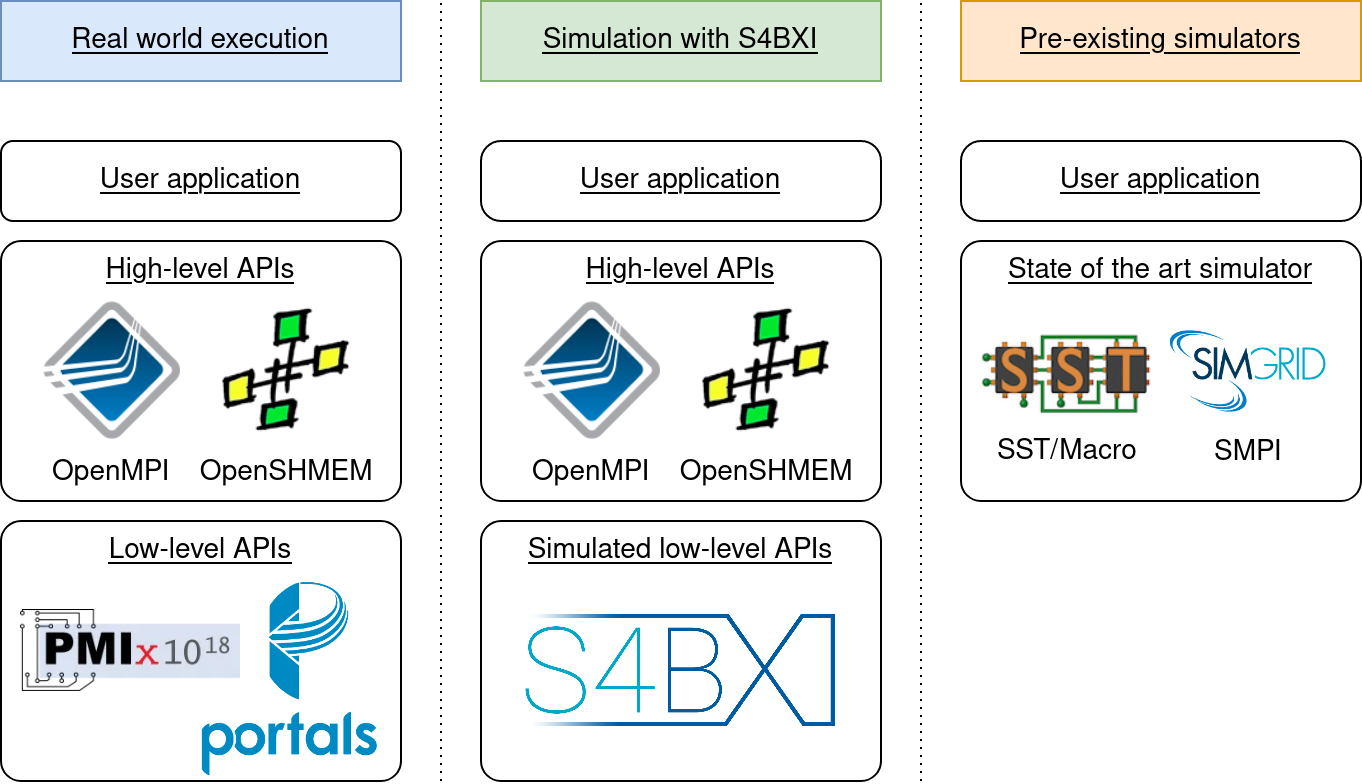
\includegraphics[width=1\textwidth]{5_high_level/software_sandwich.png}
    \caption{Software stack comparison: real world execution, S4BXI simulation and pre-existing state-of-the-art simulators}
    \label{fig:5_high_level:software_sandwich}
\end{figure}

As introduced in Section~\ref{subsec:2_context_hpc:software_stack}, a typical
software stack in HPC is made of several layers. Even though we have seen that
there are multiple possible combinations of these layers, in this section we
will focus on applications that are written directly on top of a high-level API
(in particular OpenMPI or OpenSHMEM), which uses Portals as a transport layer.
It is important to note that even though Portals is the low-level API used for
high-speed communications, high-level APIs also rely on communications across an
out-of-band network in order to initialize: indeed, it is often more convenient
to have access to a simple Ethernet network in order to exchange metadata that
will be used to set up the high-speed network. This is why high-level APIs also
use libraries such as the Process Management Interface (PMIx) for their
initialization, as they make the exchange of metadata across an out-of-band
network easier by providing primitives to perform barriers and basic data
exchanges. This software stack is represented on the left side of
Figure~\ref{fig:5_high_level:software_sandwich}.

The way this type of software stack is traditionally modeled is by intercepting
function calls at a high-level, and implementing full APIs such as MPI in
simulation directly. This is the approach which is used by state-of-the-art
simulators such as SST/Macro and SMPI, which is represented on the right side of
Figure~\ref{fig:5_high_level:software_sandwich}.

In comparison, our approach is to intercept communication primitives at Portals
level, in order to run unmodified high-level APIs on top of S4BXI, as
represented in the middle of Figure~\ref{fig:5_high_level:software_sandwich}.
There are several advantages to this approach: from a software development
perspective, implementing Portals in simulation is faster than re-implementing
all of MPI, since Portals only features point-to-point communications, whereas
MPI offers a wide range of two-sided and one-sided (RDMA) primitives, both
point-to-point and collective. Another advantage is that it allows running
different high-level APIs with a reasonable development effort, instead of
re-implementing fully every high-level API (as we will see with our OpenSHMEM
experiments, even though the majority of our work is focused on MPI). On the
other hand, there are also downsides to this approach: by running more software
layers in simulation, we expect the performance of the simulator to be worse
than higher-level models. There is also a more technical difficulty: in this
case, our low-level simulator implements Portals but we do not have a model for
PMIx (or the out-of-band network at all for that matters), which will complicate
the initialization of the high-level APIs.

The principle of our approach is to intercept communication primitives at an unusually low level in the software
stack. This method is not new and \cite{Knight2018} already implemented a similar concept, but
it has never been applied to either OpenMPI or Portals. We will see in the
upcoming sections that the technical solutions that we chose to work around the
difficulties of this approach are different from the previous approach.

\section{Atos's version of OpenMPI}
\label{sec:5_high_level:atos_ompi}

As explained previously, the most common API used on top of the BXI interconnect
is MPI, and in particular Atos's variant of OpenMPI, which we study in detail in
this PhD. While OpenMPI is a very complex set of libraries with many features,
we focus on the components that are used with BXI, which are represented in
Figure~\ref{fig:5_high_level:ompi_components}.

\begin{figure}[!ht]
    \centering
    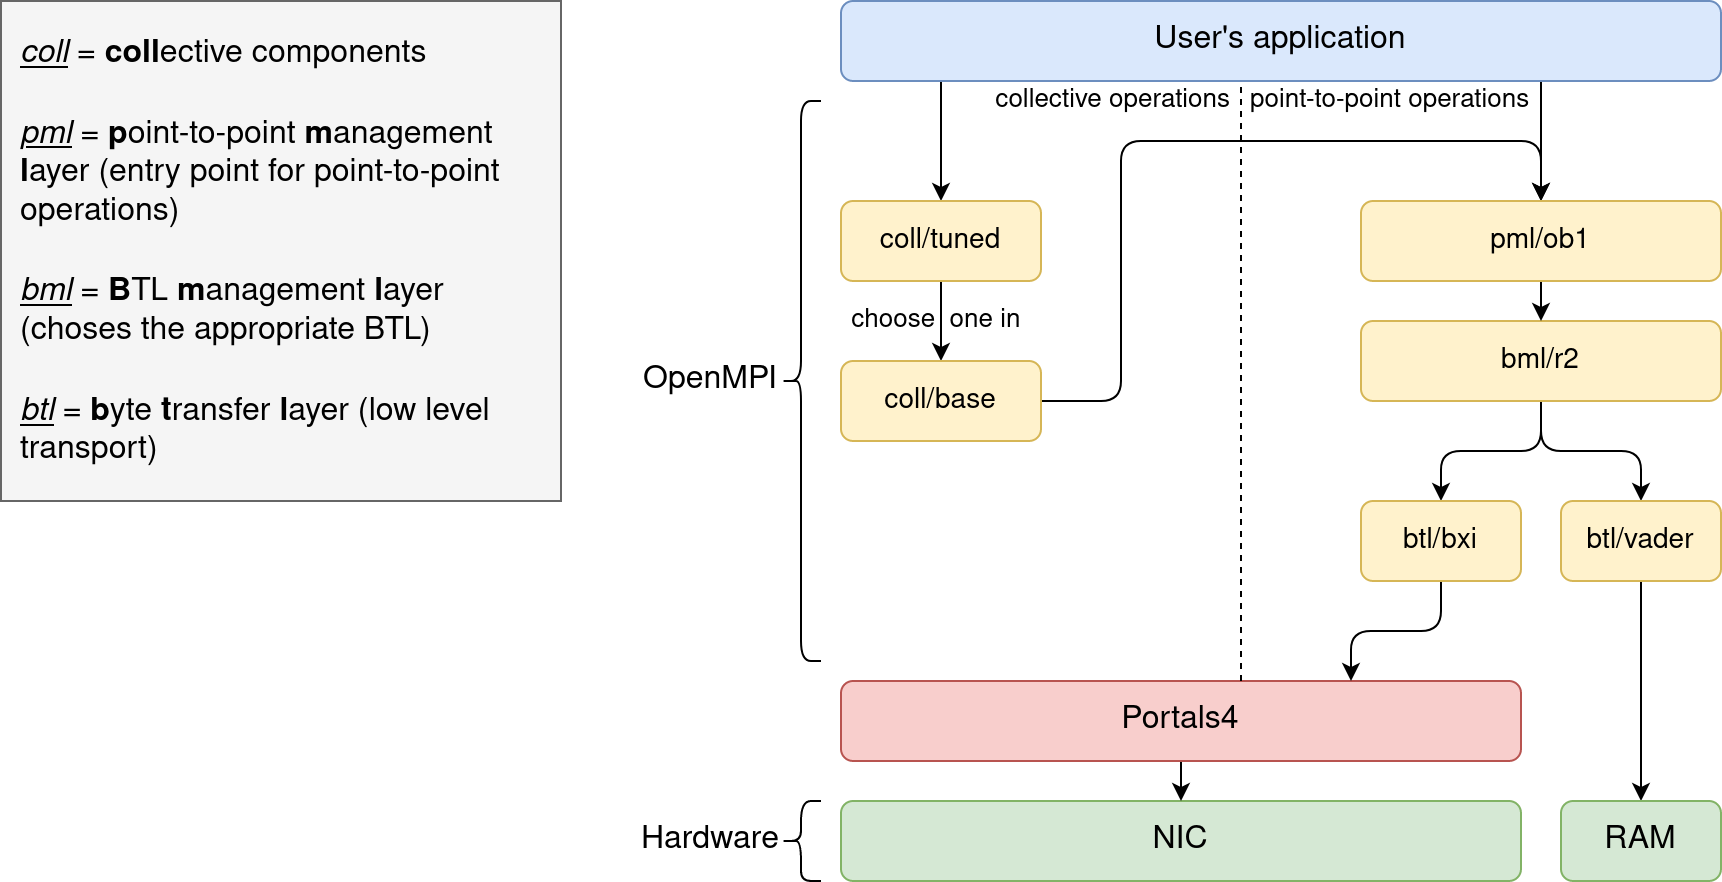
\includegraphics[width=1\textwidth]{5_high_level/ompi_components.png}
    \caption{Relevant OpenMPI components when using BXI}
    \label{fig:5_high_level:ompi_components}
\end{figure}

The components can be categorized in two main groups: collective and
point-to-point operations. Unlike Portals, MPI offers abstractions to perform
complex operations involving many processes (called ``ranks'' in MPI
vocabulary), without having the user worry about implementation details. These
operations are very diverse, such as ``gather'' (N to 1 communication),
``broadcast'' (1 to N), ``alltoall'', ``barrier'', etc. These operations all
have a synchronous and asynchronous variant, to allow users' application to
perform computations while the operation is progressing. To achieve that, the
\inline{coll/base} component implements several algorithms that perform any
given operation with a combination of point-to-point transfers (between only two
processes). Examples of a few algorithms for the broadcast operations are
displayed on Figure~\ref{fig:5_high_level:bcast_algos}, where each arrow
represents a point-to-point communication.

\begin{figure}[!ht]
    \centering
    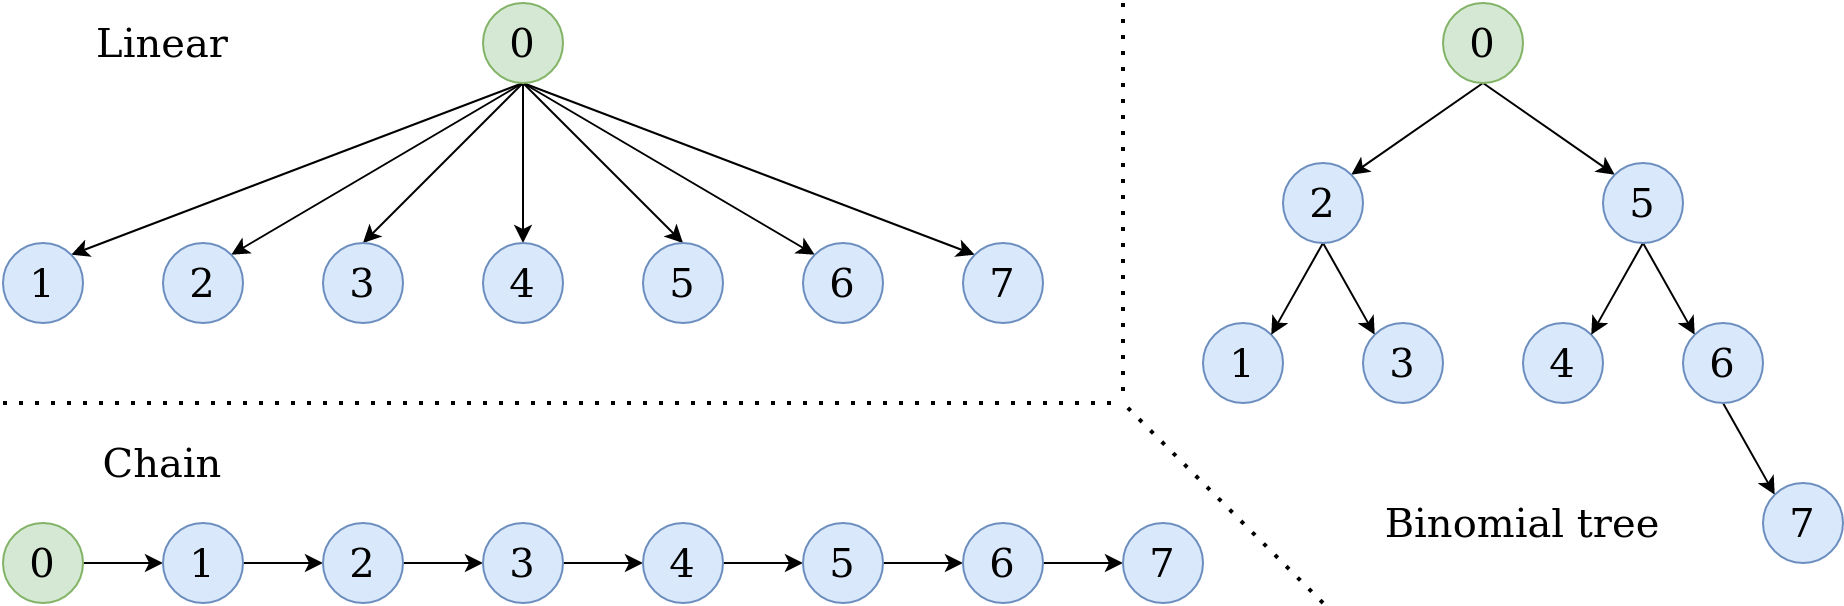
\includegraphics[width=1\textwidth]{5_high_level/bcast_algos.png}
    \caption{A few algorithm examples to perform a broadcast on 8 ranks from rank 0}
    \label{fig:5_high_level:bcast_algos}
\end{figure}

The reason different algorithms exist for each operation is to improve
performance: when the user calls a collective primitive, the
\inline{coll/tuned} component selects the algorithm to use in
\inline{coll/base} based on the number of ranks involved and the message
size. It is important to note that in the community version of OpenMPI, this
algorithm selection is based on benchmarks performed on old generation
Infiniband hardware, which is why teams at Atos made their own benchmarking
tools to optimize the algorithm choices for the BXI interconnect. Therefore,
the algorithms used in Atos's version of OpenMPI are not the same as in the
community version of OpenMPI, and still evolving (as this optimization work is
not finished as of the writing of this PhD).

When performing point-to-point operations (either from user code or as part of a
collective operation), there are three types of components that will be of
interest to us: at the highest level, the PML (Point-to-point Management Layer)
is responsible for any manipulation of the data that might be required, such as
the fragmentation of large messages. In Atos's OpenMPI the PML that we use is
called \inline{ob1} and it is not modified from the community one. Then the BML
(BTL management layer) chooses which BTL can perform the communication, based on
the location of the two ranks involved (they could run on the same machine, or
be on different nodes). The BML that we use is called \inline{r2} and it is also
identical to the community one. Finally, the BTL (Byte Transfer Layer) performs
the low-level transfer. Usually several BTLs will be used, as we can see on
Figure~\ref{fig:5_high_level:ompi_components}: for example, with the BXI
interconnect the \inline{btl/bxi} component will be used to perform
communications across the high-speed network, but the \inline{btl/vader} will be
used to perform shared memory transfers for ranks that are on the same machine.
Vader is a BTL that also comes unmodified from the community version of OpenMPI,
and BXI is entirely made by teams at Atos.

\section{Adapting OpenMPI for the simulated world}

\subsection{Simulation of out-of-band communications without PMIx}

As introduced in the previous section, the main difficulty in running a real
world MPI implementation in our simulator is the initialization: it requires
either to implement the PMIx specification in simulation, or to modify MPI
itself in order not to need this library. There are pros and cons to both
options: implementing PMIx allows running MPI with very few modifications, and
also facilitates running other high-level APIs (since PMIx is a tool commonly
used by several libraries). On the other hand, developing and maintaining a PMIx
simulator represents significant work, as it has many features. It is worth
noting that regardless of the option we choose, the accuracy of the simulator
will not be affected too much, since PMIx is only used briefly at the start and
at the end of the execution of applications. In either case we will also likely
need to rebuild MPI for simulation, since our simulator requires MPI to be built
with a specific set of options (passed to the \inline{configure} script) that
are likely different from a production build for real world executions (in
particular, we need to force OpenMPI to build into only three shared libraries,
instead of one library for each component). In the case of running Atos's
OpenMPI on top of S4BXI, we chose to add a small patch to MPI instead of
implementing PMIx, for all the reasons mentioned above. In particular, we
believe that this patch is easier to maintain than a full PMIx implementation,
and we will see in the next sections that other small modifications to MPI's
code will prove useful. A summary of the different software layers involved in
the execution of an MPI application is depicted in
Figure~\ref{fig:5_high_level:models_comparison}.

\begin{figure}[!ht]
    \centering
    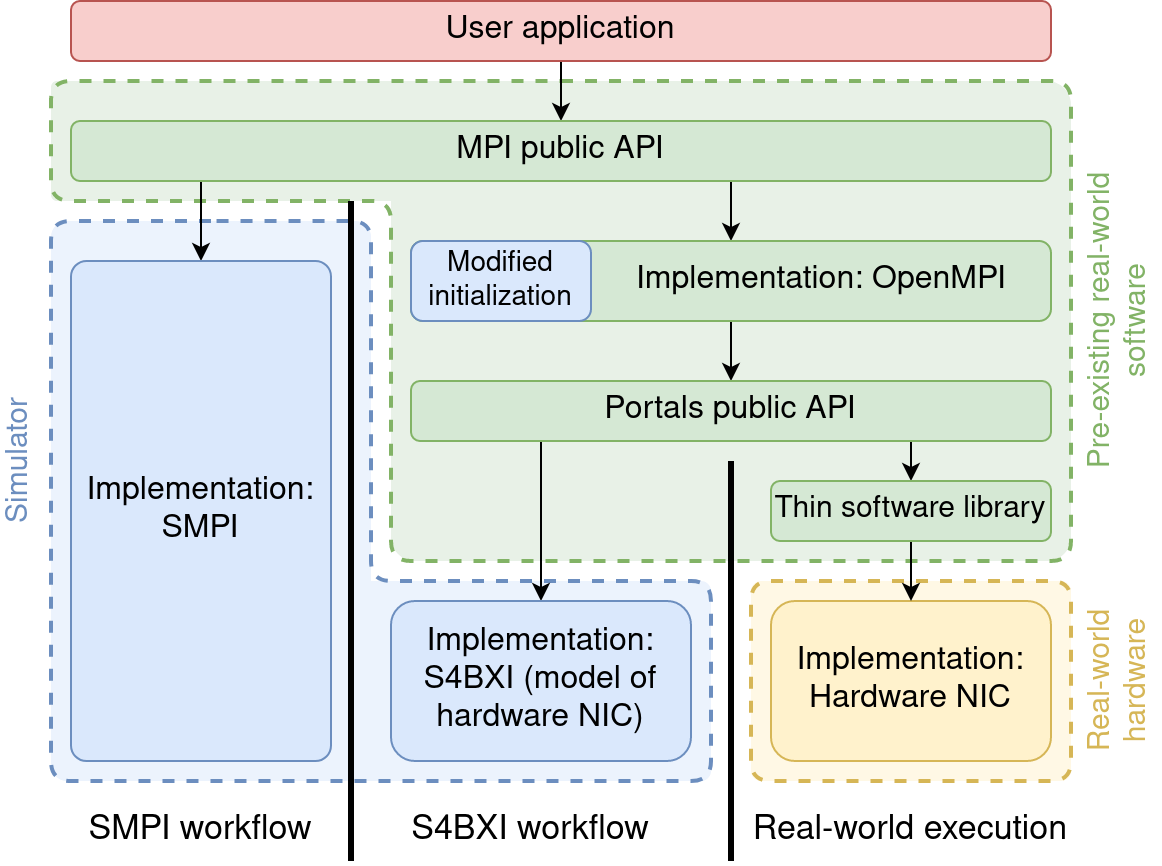
\includegraphics[width=0.8\textwidth]{5_high_level/model_comparison.png}
    \caption{Software layers involved in state of the art simulation, S4BXI simulation, and real-world execution of MPI applications}
    \label{fig:5_high_level:models_comparison}
\end{figure}

In total, our patch modifies 345 lines of code of OpenMPI: 41 lines are added,
224 are removed, and 80 are modified. This number is very small compared to the
size of the OpenMPI codebase, which contains nearly 900 thousand lines of code.
The detail of these statistics language by language are available in
Appendix~\ref{app:ompi_patch}. We also know from a year of maintaining our patch
that the code that we modified is not updated very often, as we were able to
rebase our modifications on top of the latest development to OpenMPI through
seven versions (from version 4.0.4 to 4.1.4), without any major difficulty (the
rebase through git worked automatically in the vast majority of cases). The next
sections give more detail about the components that are modified by this patch.

\subsection{Adapting OpenMPI's initialization for S4BXI}

Our patch to OpenMPI affects two main components: the initialization of MPI
itself (globally), and the initialization of the BTLs. The impacted components
are shown in Figure~\ref{fig:5_high_level:simplified_arch}.

\begin{figure}[!ht]
    \centering
    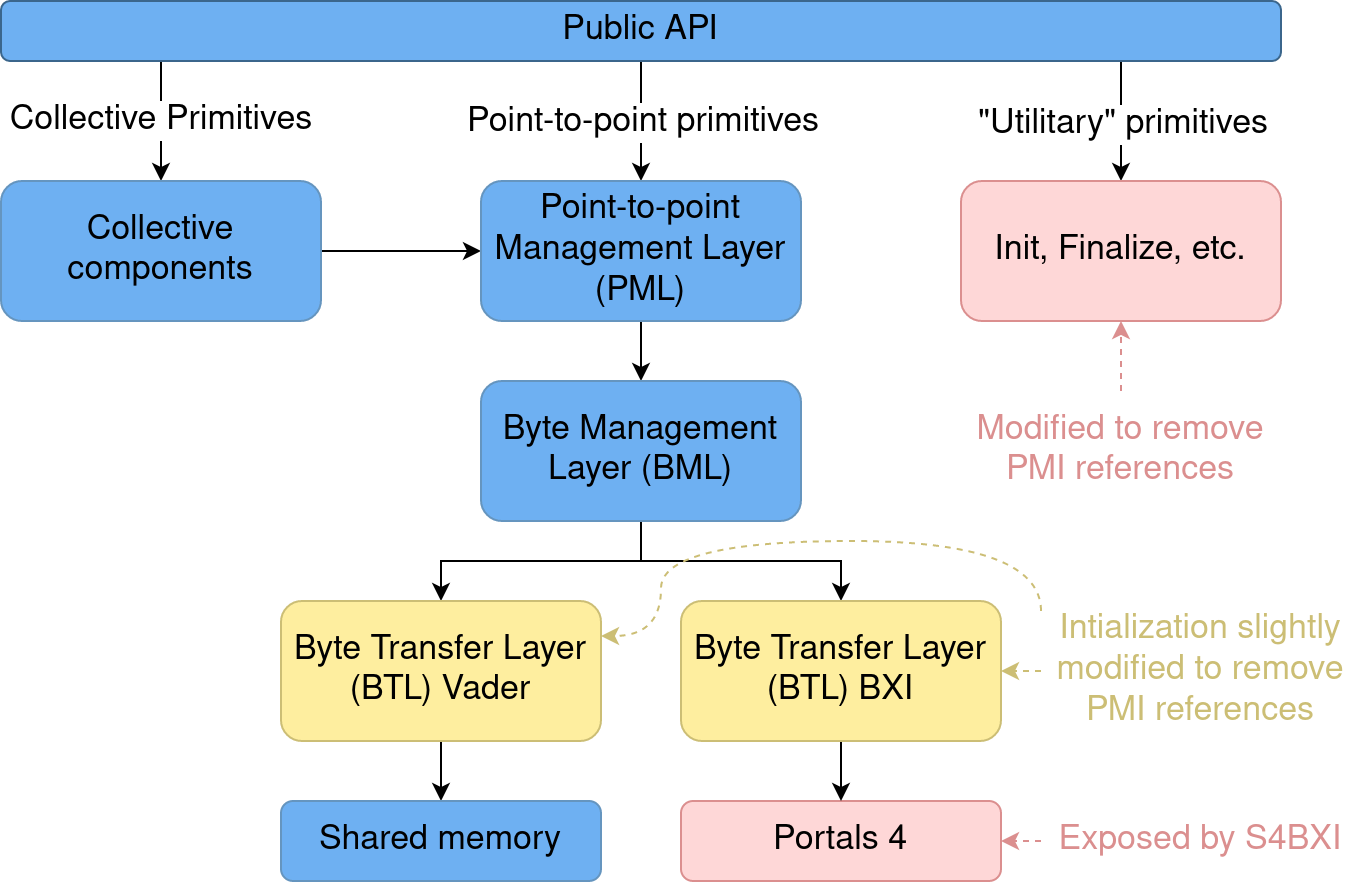
\includegraphics[width=0.75\textwidth]{5_high_level/simplified_arch.png}
    \caption{MPI components impacted by our patch \small{(dark blue is unmodified, medium yellow corresponds to minor modifications, and light red is heavily modified)}}
    \label{fig:5_high_level:simplified_arch}
\end{figure}

In the initialization of OpenMPI, we mainly replace PMIx calls to functions
native from our simulator in order to give all processes the knowledge of what
their rank is, how many processes are involved in the current job, and which
other ranks are local to the same machine. Additionally, there are a few
barriers between all the ranks that are reimplemented with SimGrid's built-in
Barrier object instead of using PMIx. An example of such replacement is shown on
Figure~\ref{fig:5_high_level:ompi_example_diff}: below several layers of macros,
\mbox{\inline{OPAL_MODEX_*}} calls use PMIx to exchange data with other
processes, so we replace them by simple function calls to our simulator which
fetch the equivalent data in the simulated world. In this specific example, the
call returns a Portals process structure (which includes a NID and a PID) for
the requested MPI rank (which correspond to the \inline{vpid} attribute
internally in OpenMPI), which is used to initialize the \inline{btl/bxi}
component.

\begin{figure}[!ht]
    \lstinputlisting[basicstyle=\ttfamily\small,frame=bt,language=diff]{5_high_level/ompi_example.diff}
    \caption{Example section of our patch to OpenMPI}
    \label{fig:5_high_level:ompi_example_diff}
\end{figure}

In the BXI BTL, the data that is exchanged at startup is mainly the Portals IDs
of each process, in particular the NIDs of all the processes involved in the
current job. At startup, the BTL also looks for all available NICs in Sysfs (in
the \inline{/sys/class/bxi} virtual folder), in order to use the closest one (in
the case of a NUMA machine). This processing had to be removed for simulation at
first, since on the host running the simulation, any BXI NIC physically present
on the machine does not correspond to the hardware simulated by our model in the
virtual world. Since then, the MPI team at Atos has been kind enough to add an
option in MPI to disable this optimization (and therefore use any available NIC
without asking for a particular location), which allows our patch to be even
lighter since we do not need to hardcode the removal of this feature.

\subsection{Shared memory support}
\label{sec:5_high_level:shared_mem_support}

As presented in Section~\ref{sec:5_high_level:atos_ompi}, MPI supports using
several BTLs for point-to-point communications. In the case of BXI clusters,
most of the time two BTLs will be used: BXI for communications on the high-speed
network, and Vader for intra-node communications using shared memory (when
several MPI ranks are executed on the same machine).

In order to support Vader in simulation, we also modified its initialization. It
is not strictly necessary in order to perform simulations of MPI (we could have
simply disabled Vader altogether), since communications between two ranks on the
same machine can still be performed trough BXI: in that case messages just go
back and forth on the PCIe bus without being sent on the network (both in a real
execution and in simulation). Nevertheless, we added support for Vader in order
to allow users to replicate their real-world scenario as closely as possible in
simulation. In theory this BTL is easy to initialize, and does not require any
data from the simulator, but in practice there is a different kind of issue with
the modeling of this BTL in simulation: by default, the name given to the files
which hold data in shared memory (in the \inline{/dev/shm} folder) can be
identical on different machines. In a real-world execution this does not matter,
as each machine will hold its own set of files, but in simulation all ranks run
on the same physical machine (which executes the simulation), which means that
different simulated processes could overwrite the data of processes on different
simulated nodes. Therefore, we had to make the name of these files unique across
the whole simulation, which required a small modification of Vader's
initialization. It is worth noting that this modification is not related to
PMIx, and therefore it further justifies our choice to patch MPI instead of
reimplementing PMIx in simulation, as this part of the patch would have been
required in any case.

\subsection{Handling copies of MPI libraries in S4BXI}
\label{sec:5_high_level:relinkage_of_libs}

Up to this point, the simple applications that we modeled did not have any
dependencies on external libraries, except Portals which is directly provided by
our simulator. Now that we try to model MPI, we face a new difficulty: as
explained in Section~\ref{subsec:4_portals:process_isolation}, we rely heavily
on the linker to isolate the global symbols of the user application in each
simulated process, but we do not have a way of isolating different copies of
external libraries (such as OpenMPI) yet. This is problematic because OpenMPI
relies heavily on global variables, which need to be ``private'' to each
simulated process. In order to tackle this issue, we can take inspiration from
SMPI: the same way that it copies the user application $N$ times (for $N$
simulated processes) in order to isolate them, it also has an option to make
multiple copies of any linked library, and then ``re-link'' the copies of the
user application and the libraries together (the current proof-of-concept
implementation uses a somewhat brutal \inline{sed} command in the copied user
applications directly). In the end, each simulated process has its own copy of
the user application, which is linked with its own copy of any library that
needs to be ``privatized'', as depicted in
Figure~\ref{fig:5_high_level:smpi_relinkage}.

\begin{figure}[!ht]
    \centering
    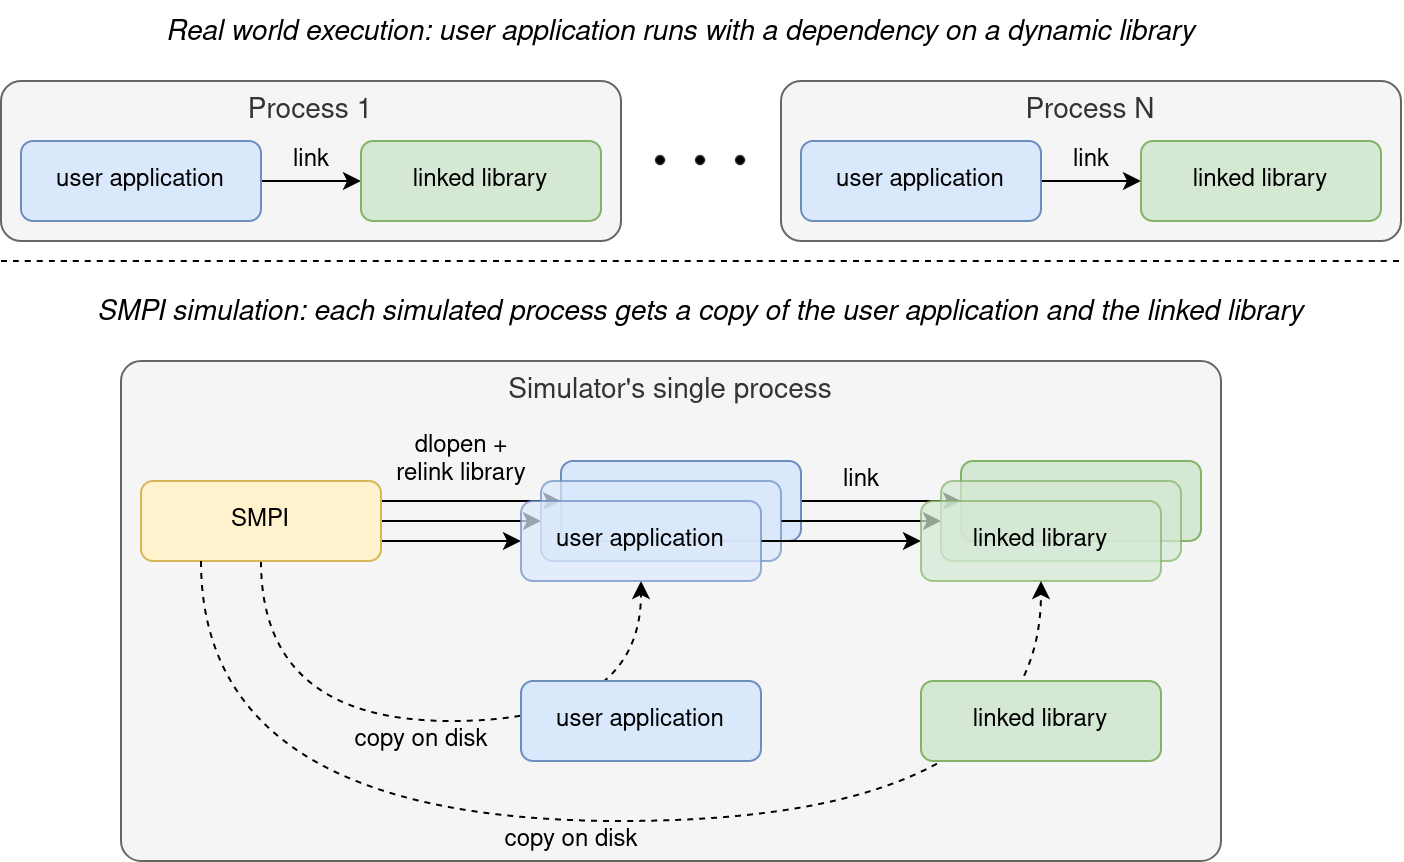
\includegraphics[width=1\textwidth]{5_high_level/smpi_relinkage.png}
    \caption{Methodology to ``privatize'' libraries in SMPI, compared to the real-world execution}
    \label{fig:5_high_level:smpi_relinkage}
\end{figure}

While this works well for libraries that are self-contained, we encountered an
issue when trying this methodology with MPI: OpenMPI does not consist of just
one library, but of three libraries (called OMPI, OPAL and ORTE), which are all
linked to the user application, but also linked to each other. Therefore, in
order for this ``privatization'' to work, we had to extend it in order to relink
not just the user application to each library, but also the copies of each
library together. This extended approach that we implemented in S4BXI is
depicted in Figure~\ref{fig:5_high_level:ompi_relinkage}.

\begin{figure}[!ht]
    \centering
    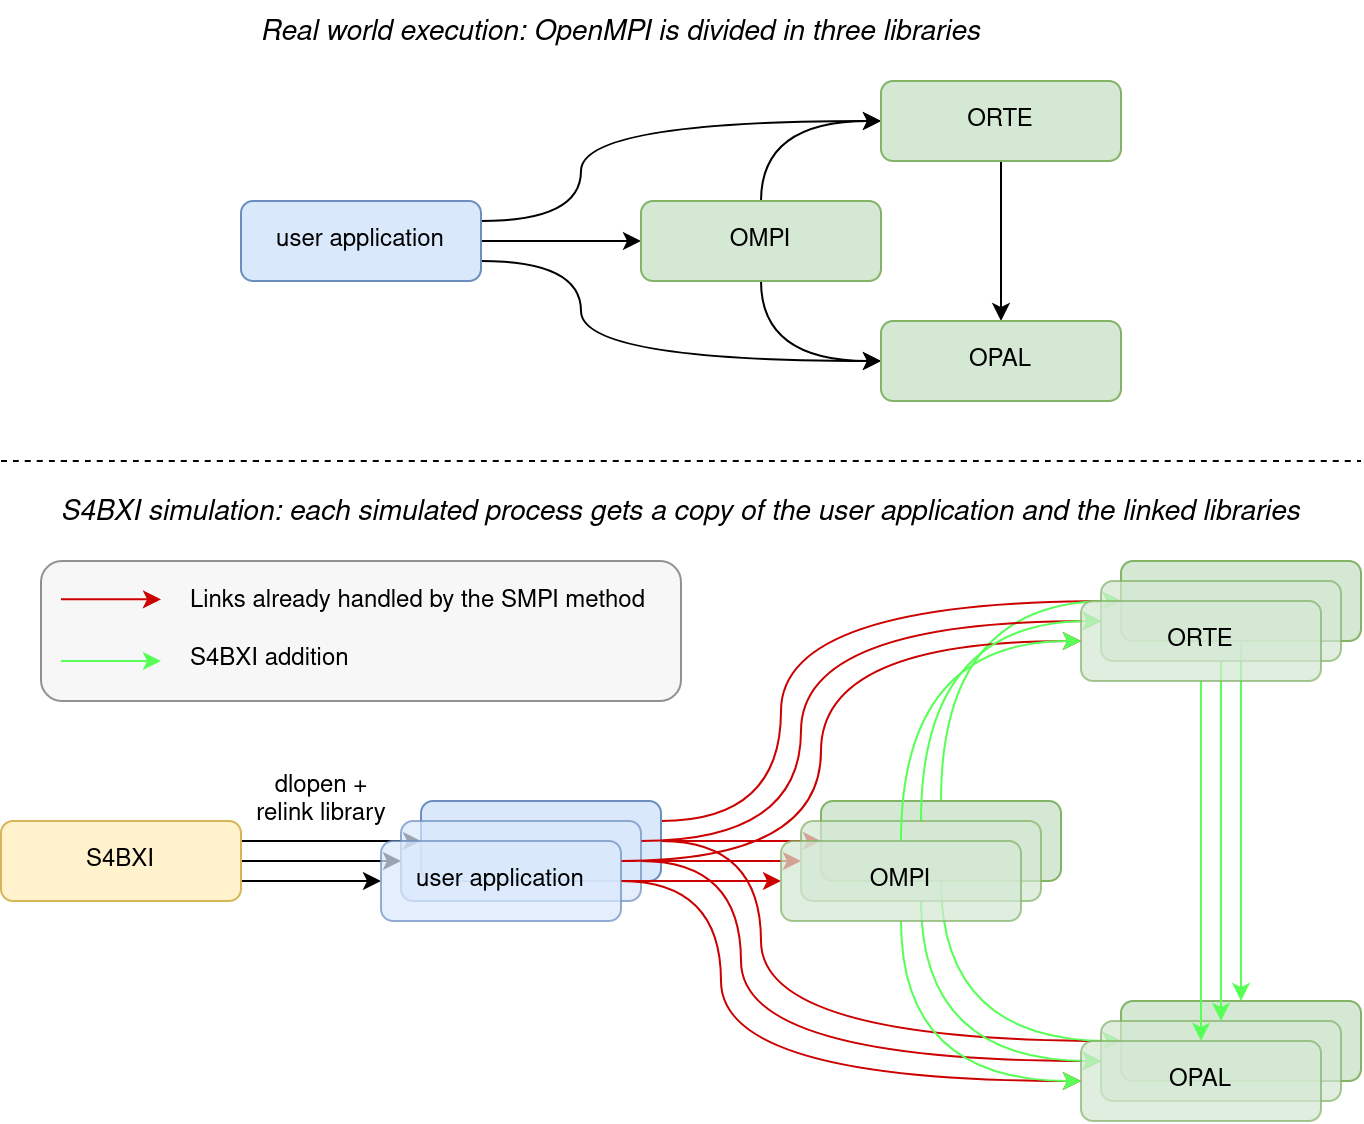
\includegraphics[width=1\textwidth]{5_high_level/ompi_relinkage.png}
    \caption{Methodology to ``privatize'' OpenMPI libraries in S4BXI, compared to the real-world execution (the ``copy on disk'' step is still present but not depicted for clarity)}
    \label{fig:5_high_level:ompi_relinkage}
\end{figure}

\subsection{A word on performance regarding polling}
\label{subsec:5_high_level:polling}

Thanks to our patch to OpenMPI, we can run simulations of real-world
applications on top of our simulator. However, we still face an issue when it
comes to performance, because of a fundamental problem with discrete event
simulators: polling. This issue was already mentioned in
Section~\ref{sec:4_portals:ptlperf}, as we observed that it impacted greatly the
performance of Ptlperf's simulations, but it is really with MPI that this
problem is the most noticeable.

In simulation, we have two different ``times'': ``wall-clock time'', during
which the user waits for the simulation to finish, and ``virtual time'', which
is a variable inside SimGrid used to keep track of the time in the simulated
world. On the other hand, on a real cluster executing a scientific application,
there is only one time: the makespan of the application. This difference becomes
very important if an application performs polling, i.e. loops over a check until
it completes. In the real world, performing polling or a ``passive'' wait is
equivalent if nothing else is running on the same CPU core. An example is
depicted on Figure~\ref{fig:5_high_level:wait_example}: while both solutions
would take the same amount of time in a real-world execution, these two programs
have a very different simulation performance.

\begin{figure}
    \centering
    \begin{subfigure}{.5\textwidth}
        \centering
        \lstinputlisting[basicstyle=\ttfamily\scriptsize,frame=bt,language=C]{5_high_level/active_polling_example.c}
        \caption{Polling around EQ Get}
        \label{fig:5_high_level:active_polling_example}
    \end{subfigure}% this comment is important otherwise the figures are vertical
    \begin{subfigure}{.5\textwidth}
        \centering
        \lstinputlisting[basicstyle=\ttfamily\scriptsize,frame=bt,language=C]{5_high_level/passive_wait_example.c}
        \caption{Passive wait with EQ Wait}
        \label{fig:5_high_level:passive_wait_example}
    \end{subfigure}
    \caption{Two ways of waiting for an event in Portals}
    \label{fig:5_high_level:wait_example}
\end{figure}

The explanation is that \inline{PtlEQWait} is cleverly implemented in our
simulator, i.e. the Actor who calls the primitives is put to sleep until the
arrival of the awaited event. On the other hand, the active polling loop of
Figure~\ref{fig:5_high_level:active_polling_example} causes an issue, because
\inline{PtlEQGet} takes a small amount of wall-clock time to simulate, but it
doesn't allow the virtual simulated time to progress. This means that when an
Actor runs such a polling loop, it will be continuously scheduled to run by
SimGrid's scheduler, but the simulated time will never progress, effectively
resulting in a deadlock of the simulation (with respect to wall-clock time).

This is a significant issue, because OpenMPI relies on polling mechanisms every
time an application asks to wait for the completion of a request (in this
context a ``request'' is to be taken in a very broad way: it could represent a
message transmission, a message reception, a collective operation, etc.). It is
worth noting that this problem is not specific to OpenMPI over Portals, but is a
common problem in discrete event simulation: if we look at simulators which
operate one level of abstraction higher in the software stack, we can see the
same problems. For example, if an application calls the \inline{MPI_Test}
primitive in a loop (which is not uncommon), SMPI will suffer the same issue.
The way SMPI handles the problem is by injecting increasing amounts of delay in
the simulated time, in the form of a small CPU execution (which is purely
artificial and does not correspond to real computation).

\begin{algorithm}
    \caption{OpenMPI's algorithm to wait for the completion of a request}
    \hspace*{\algorithmicindent} \textbf{Input} $request$ a pending request, $BTL$ the list of BTLs in use, $N$ the number of BTLs
    \begin{algorithmic}[1]
    \While{$request$ is not complete}
        \For{$i \gets 0$ to $N - 1$}
            \State{progress\_btl\_number($i$)}
        \EndFor
    \EndWhile
    \end{algorithmic}
    \label{alg:5_high_level:ompi_wait}
\end{algorithm}
\begin{algorithm}
    \caption{Algorithm~\ref{alg:5_high_level:ompi_wait} applied to our specific case}
    \hspace*{\algorithmicindent} \textbf{Input} $request$ a pending request
    \begin{algorithmic}[1]
    \While{$request$ is not complete}
        \State{progress\_btl\_BXI()}
        \State{progress\_btl\_vader()}
    \EndWhile
    \end{algorithmic}
    \label{alg:5_high_level:ompi_wait_specific}
\end{algorithm}

Initially, we resolved this issue in our simulation with a better approach: by
analyzing the code of OpenMPI, we were able to find a heuristic to determine
when it was safe to perform a Portals EQ Wait (i.e. blocking wait) instead of a
loop over an EQ Get. This allowed us to keep an accurate simulation while
speeding it up by orders of magnitude. Unfortunately, this solution only worked
well at the time when we supported only the BXI BTL in simulation. Indeed,
internally the algorithm used to wait for the completion of a request roughly
follows Algorithm~\ref{alg:5_high_level:ompi_wait}, where the PML will loop over
each BTL and call its ``progress'' function until the request is complete. The
``progress' function of a BTL typically runs every callback that is ready in the
context of asynchronous operations, and checks for new events coming from the
underlying transport. When we supported only one BTL, it was easy to replace the
progress function by a blocking wait. Unfortunately, when we added support for
shared memory transfers using the vader BTL, this optimization stopped working,
because the completion of a request could now come from any of the two BTLs, as
depicted in Algorithm~\ref{alg:5_high_level:ompi_wait_specific}. In the general
case it is not possible to know from which BTL the completion of a request will
come, because of how generic a request is in this part of a code. Additionally,
our problem was further complicated by the fact that some options of OpenMPI
require progress functions to run as often as possible: for example, it is
possible to turn on flow control for the BXI BTL of OpenMPI, in which case if
too many messages are already inflight, new ones will wait in a queue (in order
not to flood a target). It is then in the progress function of the BXI BTL that
a check will be performed to see if pending messages can be sent. Therefore,
having a blocking wait in this function stops this check from working properly,
since it might get scheduled too late, or not at all in the worst situations.

This problem further reduces the number of cases in which our heuristic to
improve performance works, and therefore we abandoned it completely: in the
latest versions of our simulator, we implement the same mechanism as SMPI in
S4BXI, i.e. injecting growing amounts of delay inside \inline{PtlEQGet} to make
sure that a polling loop can still allow the simulated time to progress at a
reasonable rate (this small delay is configurable using the environment variable
\inline{S4BXI_ACTIVE_POLLING_DELAY}).

\section{Compatibility with SMPI sampling}

When running applications in simulation, one of the biggest concern is the
memory usage and the performance of the simulator: indeed, most simulators built
with SimGrid are single-threaded, which means that all processes of the
application end up being executed sequentially on one CPU core. To mitigate this
issue, SMPI offers a set of macros in order to replace some heavy computation
parts with increments in the simulated time. The amount of computation time to
inject can be statically provided by the user, or determined automatically at
runtime, thanks to macros which replace \inline{for} loops. These macros allow
SMPI to execute the first iterations of the loop in order to measure their
duration, and to replace the later ones with artificial computation time. For
memory usage, SMPI allows users to mark some memory allocation as ``shared'',
which means that all simulated process will use the same physical memory region
instead of all doing a new allocation. Of course this generally makes the result
of computations functionally wrong, but for applications in which the control
flow does not depend on the input data it is a good solution to run full size
applications in simulation and get good performance estimations. These macros
effectively allow users to make skeleton version of their application, in order
to speed up simulation and allow it to run on a single CPU.

In S4BXI, we are able to re-use all these SMPI macros transparently, since both
simulators are based on SimGrid. This allows us to re-use studies that have been
conducted on specific applications in order to create optimized skeleton
versions. For example, Tom \textsc{Cornebize}'s thesis~\cite{Cornebize2021}
studied HPL extensively, and we re-used his model of HPL's computation phases in
order to speed up S4BXI simulations by orders of magnitude. This will be
demonstrated in our validation experiments in
Section~\ref{sec:5_high_level:benchmarks}.

\section{Experimental validation}
\label{sec:5_high_level:benchmarks}

While most applications can be run using both MPI and OpenMP parallelization
(sometimes even CUDA), in our experiments we will distribute them using MPI
only, as our simulator does not support arbitrary OpenMP (nor CUDA) code. This
is a common limitation which is present in similar simulators as well (such as
SMPI for example). There is a priori no fundamental limitation that would
prevent us from developing a model for OpenMP or CUDA, but such a development is
way beyond the scope of this thesis.

We will start with OSU micro-benchmarks, which are a set of
very simplistic ``unit-style'' tests that benchmark a single primitive in a
loop. While the resulting workload is completely unrealistic, it is a common
tool to assess the performance of a cluster on a specific MPI primitive, and it
is also a good validation that all collective and point-to-point operations work
without errors in simulation. We will then study realistic applications that we
presented in Chapter~\ref{chap:biblio_simu}: LULESH, Quicksilver and HPL.

From a technical perspective, all our benchmarks will be executed on a
real-world cluster composed of nodes equipped with BXI v2 hardware and AMD EPYC™
7763 64-Core processors. In simulation, we will run each application both in our
model (with OpenMPI on top of S4BXI), and in SMPI, in order to compare our
approach to the closest state-of-the art simulator.

\subsection{OSU micro-benchmarks}
\label{subsubsec:5_high_level:osu_results}

For these experiments, we will run point-to-point benchmarks on two machines,
and collective operations on 16 machines, with only one process on each machine
in order to maximize the network load. Experiments were also performed on 32 MPI
ranks (8 nodes and 4 processes per node), but the conclusions where very
similar, therefore this data is only shown in Appendix~\ref{app:osu_32} to keep
this section more readable. The simulations are performed on one of the machines
from the real-world cluster, with an AMD EPYC™ 7763 64-Core processor (even
though only one core of the processor is used in each simulation). Since OSU
micro-benchmarks cover many MPI primitives, it is impractical to analyze the
result of each simulation exhaustively. Instead, we present a few significant
experiments, but we also show global statistics about all the simulations.

Across all benchmarks, we get mainly two types of results. In some cases, both
SMPI and OpenMPI over S4BXI give very good results (i.e. latencies reported by
the benchmark at the end of its execution). We can see  an example of such a
behavior with the AllGather benchmark, depicted on
Figure~\ref{fig:5_high_level:osu_allgather_16} (AllGather allows all processes
to send chunks from a local buffer to all the other processes in the job).

\newgeometry{top=2.2cm,footskip=0.8cm}
\begin{figure}[!p]
    \centering
    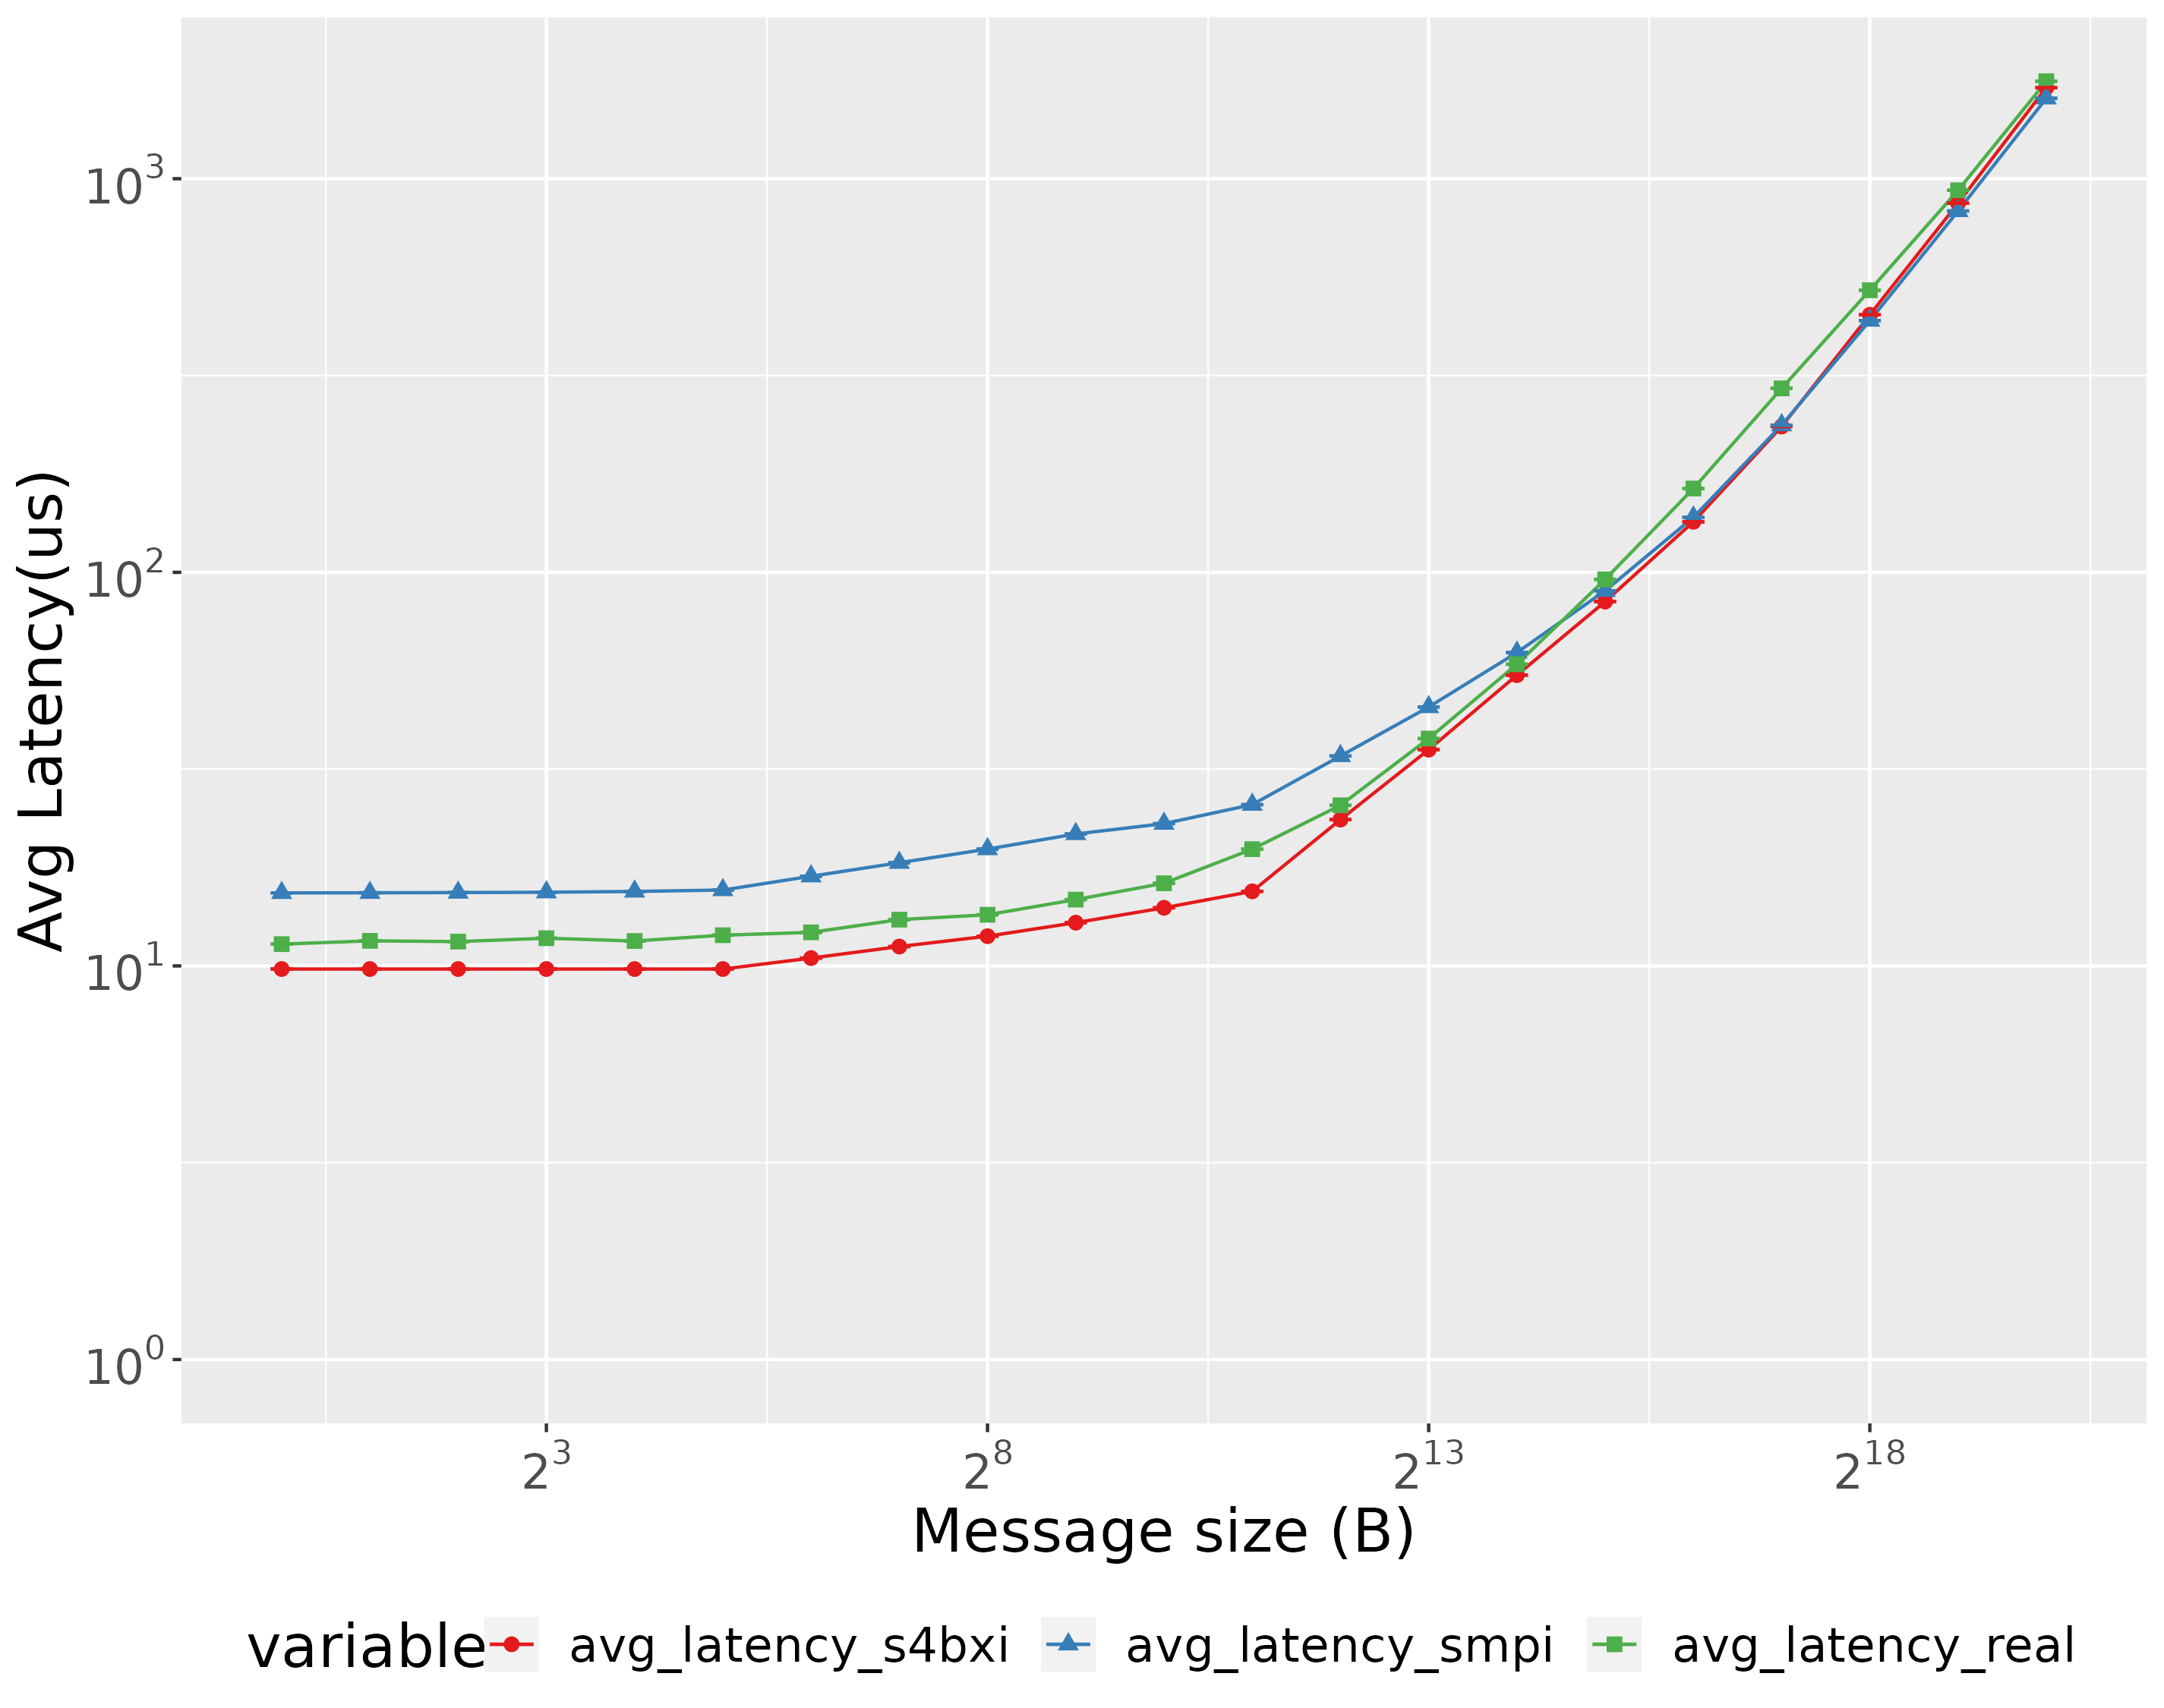
\includegraphics[width=0.88\textwidth]{5_high_level/OSU/allgather_16.png}
    \caption{OSU AllGather benchmark: comparison between the real-world run, an SMPI simulation, and an OpenMPI over S4BXI simulation}
    \label{fig:5_high_level:osu_allgather_16}
\end{figure}

\begin{figure}[!p]
    \centering
    \includegraphics[width=0.88\textwidth]{5_high_level/OSU/reduce_16.png}
    \caption{OSU Reduce benchmark: comparison between the real-world run, an SMPI simulation, and an OpenMPI over S4BXI simulation}
    \label{fig:5_high_level:osu_reduce_16}
\end{figure}
\restoregeometry

In other cases, we can see a significant loss of accuracy for SMPI, usually for
specific message size. We can see an example of such a behaviour with the Reduce
benchmark, depicted on Figure~\ref{fig:5_high_level:osu_reduce_16}. Reduce
allows a ``root'' process to synthesize values from all processes into a single
value, by applying an arithmetic operation (for example a sum, taking the
maximum, etc.). In these cases, SMPI lacks accuracy because its implementation
of the collective operation does not match the algorithm used in Atos's version
of OpenMPI. Therefore, the sequence of point-to-point transfers that are
simulated is not an accurate model for the real-world benchmark, whereas in
S4BXI  we run the real-world MPI implementation  in our simulator. Consequently,
we get a realistic model of collective algorithms because of our simulation
method.

\begin{figure}[!ht]
    \centering
    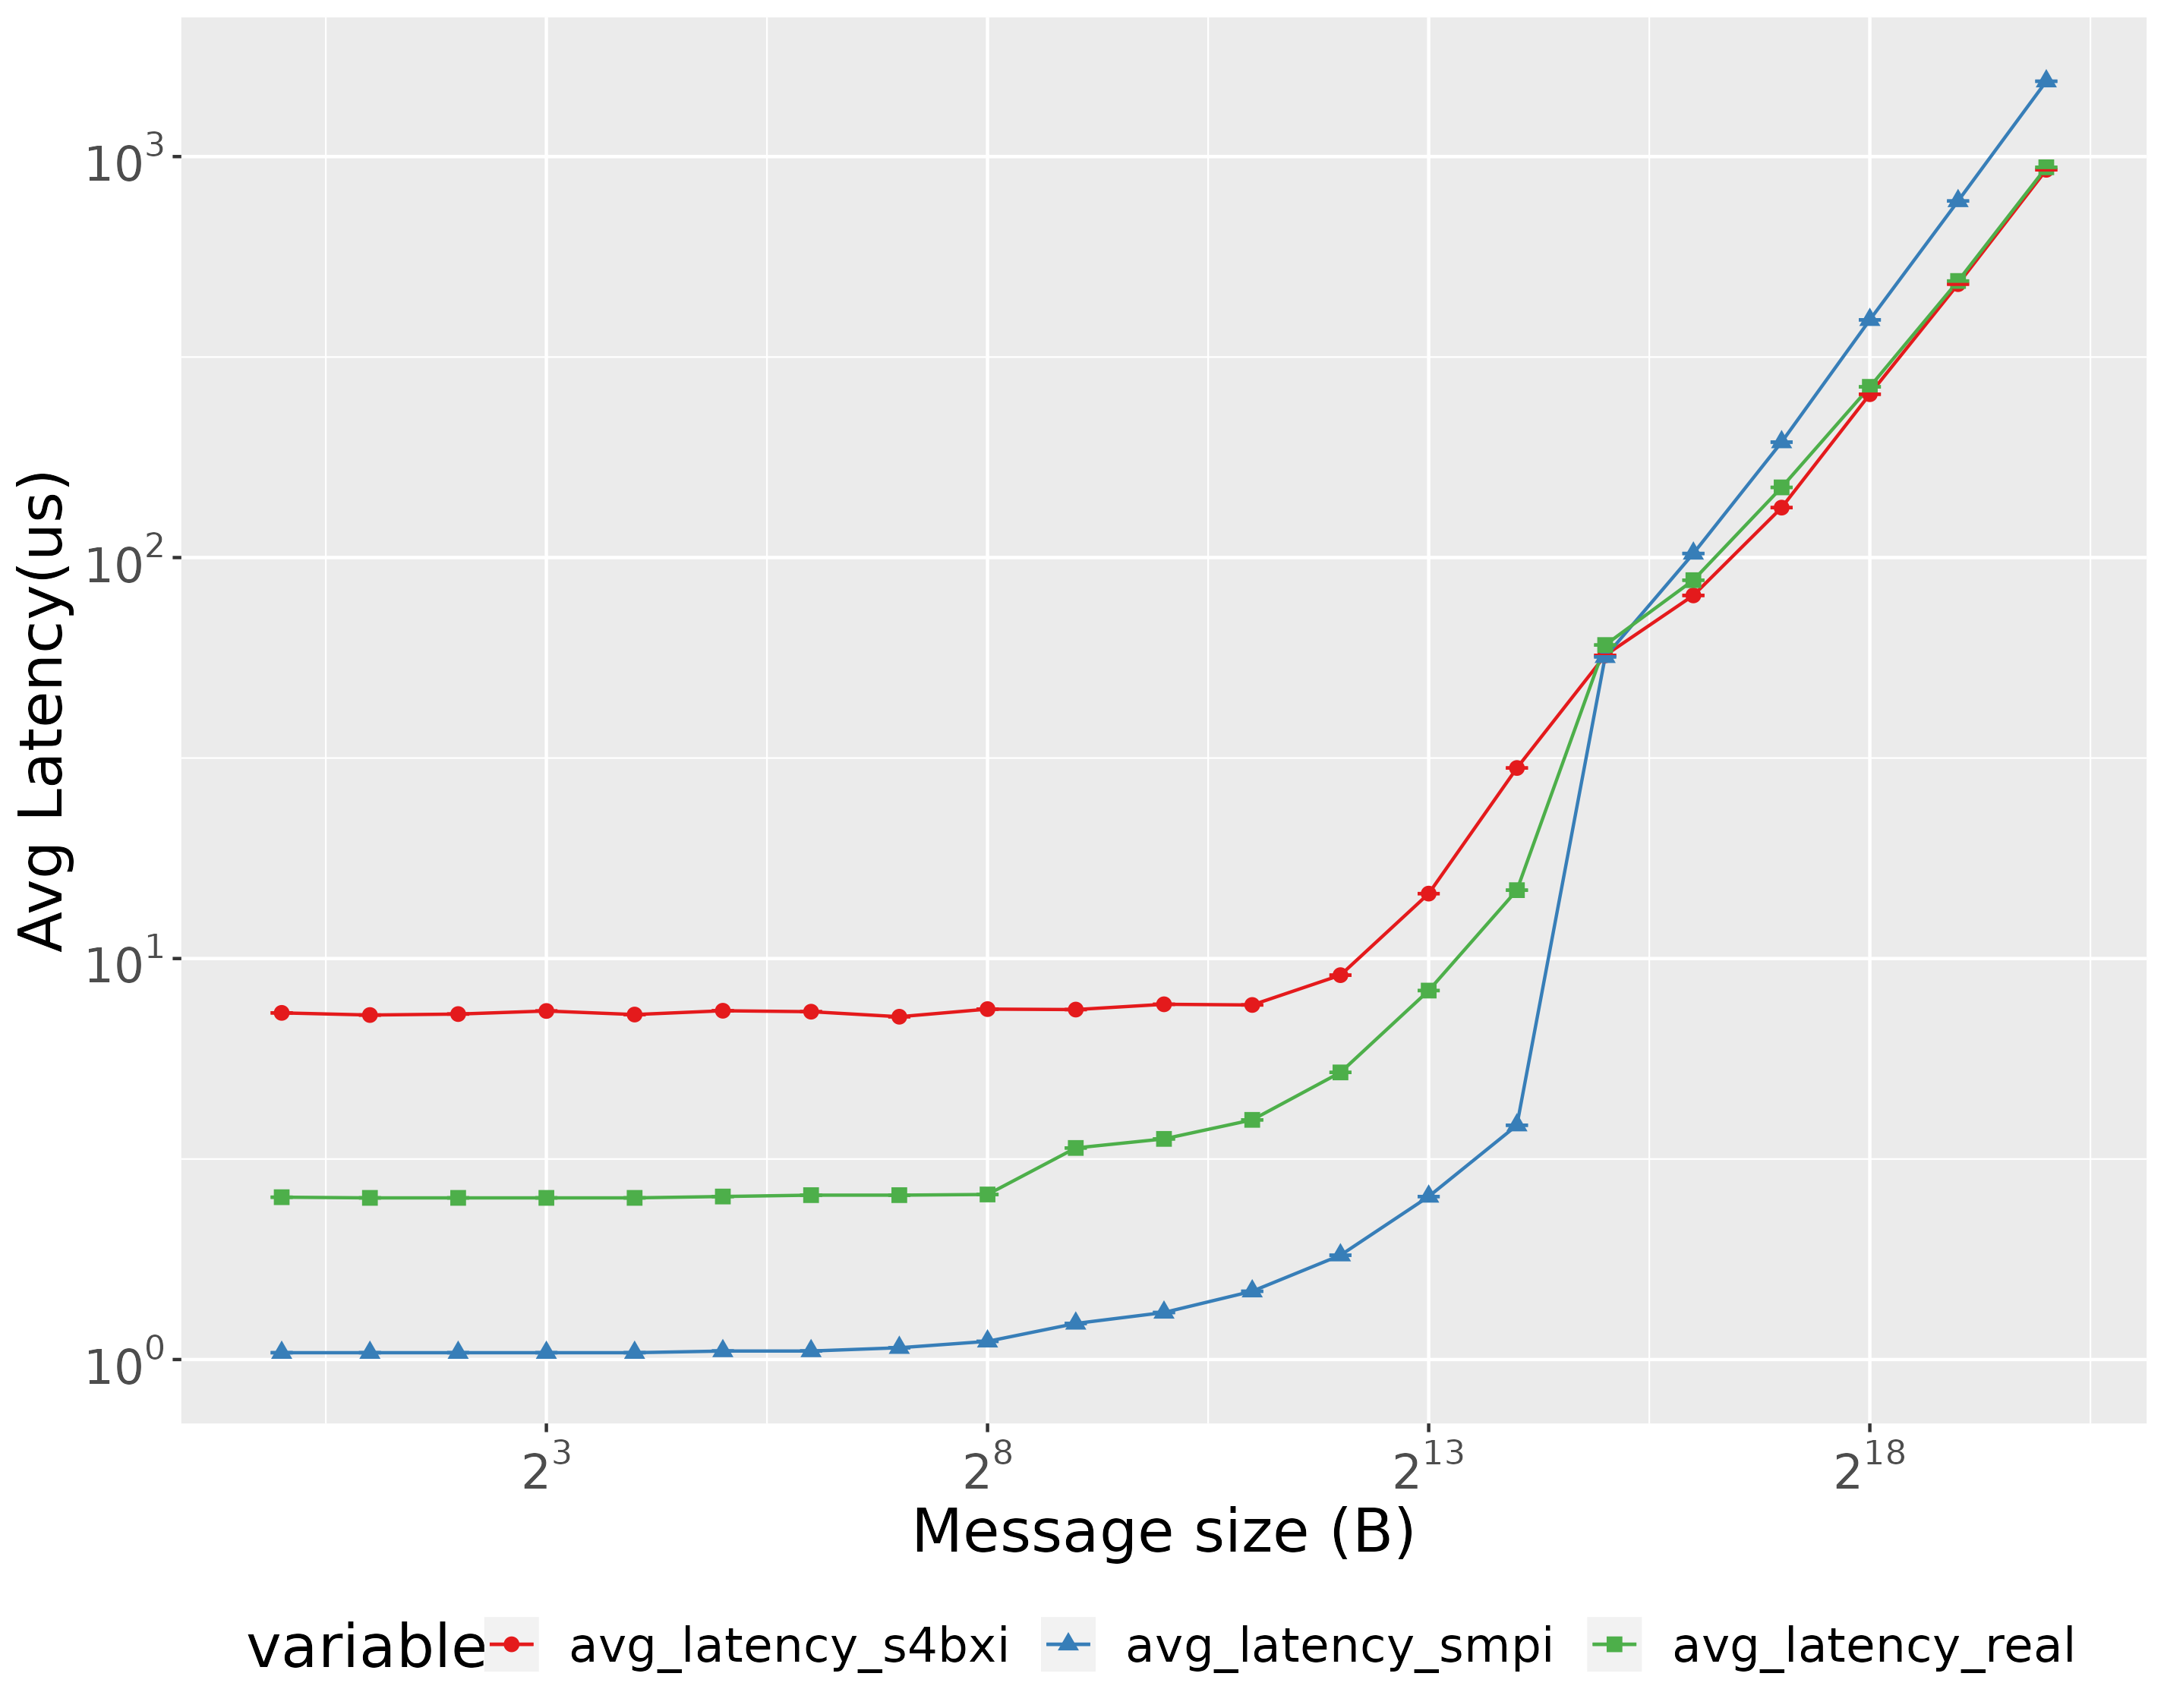
\includegraphics[width=0.88\textwidth]{5_high_level/OSU/gatherv_16.png}
    \caption{OSU GatherV benchmark: comparison between the real-world run, an SMPI simulation, and an OpenMPI over S4BXI simulation}
    \label{fig:5_high_level:osu_gatherv_16}
\end{figure}

Finally, there is one benchmark in particular that is particularly pathologic
for our simulation method: GatherV, which is depicted on
Figure~\ref{fig:5_high_level:osu_gatherv_16}. GatherV allows a ``root'' process
to fetch values from all processes, using non-continuous buffers. In this
experiment, OpenMPI over S4BXI is too pessimistic, while SMPI is too optimistic
but to a lesser degree. These results are very similar with the asynchronous
variant of this collective operation, IGatherV. These results are unusual
compared to the majority of our simulations, but we did not investigate them in
depth for two reasons. First, because of a lack of time, but also because we did
not encounter these operations in any of the applications that we executed in
simulation.

In order to get a more general view of our results compared to SMPI, we plotted
the average error of each simulation, by computing the absolute difference
between our simulation result and the value from the real-world experiment, and
averaging these values across all message sizes. The resulting graph is shown on
Figure~\ref{fig:5_high_level:osu_errors}.

We can see the three different patterns that we presented. First, most
simulations are of a similar accuracy in both approaches. In several other cases
simulations are significantly more precise in OpenMPI over S4BXI. Finally, there
are still a few operations for which both simulators have a high error, in some
of these cases our simulation method has an even larger error than SMPI, but
these cases are rare.

From a performance perspective, we can see on
Figure~\ref{fig:5_high_level:osu_perf} the slowdown of running a simulation
compared to performing an execution on a real-world cluster. Most of the time,
simulators are two orders of magnitude slower than real-world executions (around
100 times slower). This result is expected, as OSU benchmarks are extremely
communication-intensive, and therefore they stress our simulators to the
maximum. This figure also shows that S4BXI is generally slower than SMPI, which
comes from our architecture with more software layers, but the slowdown of our
approach is still of the same order of magnitude as state-of-the-art simulators.
In some rare cases, our approach even manages to be slightly faster, for
operations that are particularly costly to model in SMPI.

\begin{figure}[!hb]
    \centering
    \includegraphicsOverflow{5_high_level/OSU/OMPI_smpirun_16nodes1ppn_all.png}{1.2}
    \caption{Average error of both simulators: SMPI compared to OpenMPI over S4BXI}
    \label{fig:5_high_level:osu_errors}
\end{figure}

\begin{figure}[!hb]
    \centering
    \includegraphicsOverflow{5_high_level/OSU/OMPI_smpirun_16nodes1ppn_all_perf.png}{1.2}
    \caption{Average slowdown of both simulators compared to the real-world execution}
    \label{fig:5_high_level:osu_perf}
\end{figure}

\subsection{LULESH}

LULESH is a proxy application that is commonly used to assess the performance of
a cluster. In particular, it is frequently used to benchmark BXI, which is why
it is an interesting application to run in our model. As presented in
Section~\ref{subsubsec:2_context_hpc:LULESH}, LULESH has a few requirements: it
can only run on a number of MPI ranks that is the cube of an integer, for
example 1, 8, 27, 64, etc. processes. In our case, we are going to run this
application with 1 rank, 8 ranks on 8 machines (1 rank per machine), and 27
ranks on 9 machines (3 ranks per machine).

Each real-world experiment and each simulation is executed five times in order
to check the consistency of our results. LULESH is also executed for eleven
different problem sizes, which gives us executions that range from 0.15 seconds
up to a bit over a minute on the real-world cluster.

\begin{figure}[!ht]
    \centering
    \includegraphicsOverflow{5_high_level/LULESH/s4bxi_smpirun_no_vader_1ranks.png}{1.1}
    \caption{LULESH results on one MPI rank, comparing our simulator, SMPI, and a real-world execution (left graph shows accuracy, right graph shows performance)}
    \label{fig:5_high_level:s4bxi_smpirun_no_vader_1rank}
\end{figure}

Results are displayed for 1 MPI rank on
Figure~\ref{fig:5_high_level:s4bxi_smpirun_no_vader_1rank}, for 8 MPI ranks on
Figure~\ref{fig:5_high_level:s4bxi_smpirun_no_vader_8ranks}, and for 27 MPI
ranks on Figure~\ref{fig:5_high_level:s4bxi_smpirun_no_vader_27ranks}. The
simulation for only one process does not give us any information on the validity
of our network model, as there is no network communication, but it is a good
reference point to validate two things: first, that our model of computations
gives us accurate results, and second, that the performance of the simulators in
this scenario is good (that the overhead of running the application in
simulation is small). We can see on
Figure~\ref{fig:5_high_level:s4bxi_smpirun_no_vader_1rank} that these two
properties are indeed correct for both S4BXI and SMPI: on the left side, we can
see the time reported by LULESH at the end of its execution, which allows us to
assess the accuracy of the simulators. On the right side, we can see the
performance of the simulators compared to the execution time of the real-world
run. Both graphs show that the simulators are very close to the
real-world run.

\begin{figure}[!ht]
    \centering
    \includegraphicsOverflow{5_high_level/LULESH/s4bxi_smpirun_no_vader_8ranks.png}{1.1}
    \caption{LULESH results on 8 MPI ranks (8 nodes, 1 ranks per node), comparing our simulator, SMPI, and a real-world execution (left graph shows accuracy, right graph shows performance)}
    \label{fig:5_high_level:s4bxi_smpirun_no_vader_8ranks}
\end{figure}

On the other hand, on
Figure~\ref{fig:5_high_level:s4bxi_smpirun_no_vader_8ranks}, we can see the
result of an execution on 8 nodes (with 1 process per node), and the
corresponding simulations. We can see that the accuracy of both simulators is
still excellent, as they are very close to our reference values from the
real-world on all problem sizes. From a performance point of view, both
simulators are significantly slower than the real-world execution. This result
is expected, since all eight simulated processes are executed sequentially in
these single-threaded simulators (and therefore we expect a slowdown of at least
a factor of eight). We can also see that the S4BXI approach is slower than SMPI,
which once again is expected, since running a full OpenMPI implementation on top
of Portals is slower than running an MPI implementation that was specifically
optimized to run in SimGrid.

\begin{figure}[!ht]
    \centering
    \includegraphicsOverflow{5_high_level/LULESH/s4bxi_smpirun_no_vader_27ranks.png}{1.1}
    \caption{LULESH results on 27 MPI ranks (9 nodes, 3 ranks per node), comparing our simulator, SMPI, and a real-world execution. Vader is disabled in real-world OpenMPI and OpenMPI over S4BXI}
    \label{fig:5_high_level:s4bxi_smpirun_no_vader_27ranks}
\end{figure}

Finally, the execution on 27 ranks (with 9 nodes and 3 processes per node)
allows us to test further the network model of each simulator, and also to make
sure that intra-node communications give accurate results. As presented in
Section~\ref{sec:5_high_level:shared_mem_support}, intra-node communications can
be performed in two different ways: either using the Vader BTL, or simply by
going through Portals. Of course, enabling Vader to perform communications
across shared memory is irrelevant in SMPI, as it does not feature such
low-level configuration options. The results are displayed on
Figure~\ref{fig:5_high_level:s4bxi_smpirun_no_vader_27ranks} with Vader disabled
on the real-world execution and OpenMPI over S4BXI, and on
Figure~\ref{fig:5_high_level:s4bxi_smpirun_vader_emulated_27ranks} with Vader
enabled. We can see that the results are very similar in both cases, and that
our two simulators perform well regardless of whether we use Vader or not. The
reason why the performance of LULESH is identical whether we use Vader or not,
comes from the efficiency of BXI NICs. Indeed, when Portals is used to transfer
data between two processes on the same machine, the NIC effectively acts as a
DMA controller, which copy the payload from the source buffer of the sender
process to the reception buffer of the target process. This is very similar to
how Vader operates, using shared memory to copy data between processes,
therefore it is expected to observe a similar performance. Once again, we see a
considerable loss of performance compared to the execution on 8 processes, which
corresponds to what we expected (as we now run 27 MPI ranks in a single thread
in our simulators).

\begin{figure}[!ht]
    \centering
    \includegraphicsOverflow{5_high_level/LULESH/s4bxi_smpirun_vader_emulated_27ranks.png}{1.1}
    \caption{LULESH results on 27 MPI ranks (9 nodes, 3 ranks per node), comparing our simulator, SMPI, and a real-world execution. Vader enabled in real-world OpenMPI and OpenMPI over S4BXI}
    \label{fig:5_high_level:s4bxi_smpirun_vader_emulated_27ranks}
\end{figure}

The conclusion of this experiment is that while both simulators have a very good
accuracy when running LULESH, our approach does not offer any benefit over SMPI,
as the accuracy is similar, and the performance inferior. This result is not
very surprising, as LULESH relies heavily on point-to-point communication (with
little collective operations). Since SMPI is calibrated specifically on these
point-to-point primitives, it is expected to get very good results, and these
experiments validate that our calibration of the network parameters of SMPI is
accurate too.

\subsection{Quicksilver}
\label{subsec:5_high_level:quicksilver}

Quicksilver is an application that performs ten independent cycles of
computations on a configurable number of particles. At the end of the execution,
Quicksilver reports three performance values for each cycle of computations: the
time taken by the initialization, the ``tracking'' phase (where most
computations happen), and the finalization of the cycle. In practice, we have
observed that the initialization and finalization phase of each cycle have a
duration which is negligible compared to the ``tracking'' phase, therefore we
will only show the tracking times of each cycle in our graphs, for more clarity.
We have run Quicksilver for different particle numbers, ranging from 10,000 up
to 1,000,000, and many cluster configurations: we used platforms with all
combinations of 1, 2, 4, 8 and 16 nodes with 1, 2 and 4 processes per node.
Since the resulting graphs are very numerous, in this section we will present a
few representative cases of the types of results we obtained.

From a technical point of view, the simulations were performed on one of the
machines from the real-world cluster, with an AMD EPYC™ 7763 64-Core processor.
Every real-world execution was executed five times, and each simulation was
executed twice (because of a lack of time towards the end of this thesis).
Additionally, once again we had the choice of enabling Vader or not when using
several processes per node. We observed little difference with and without Vader
in our results (both in simulation and the real world experiments), therefore we
will only present experiments performed without Vader, in order to reduce the
number of variables to analyze in this section.

\begin{figure}[!b]
    \centering
    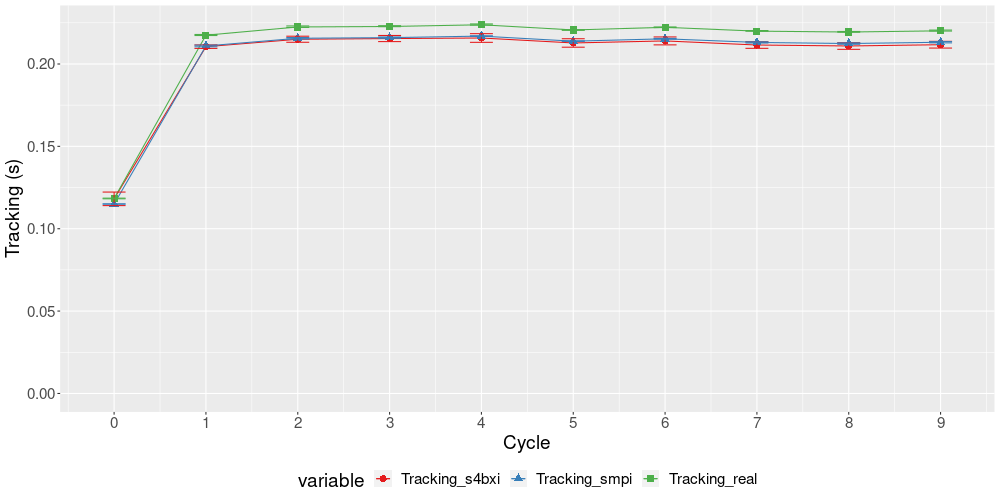
\includegraphics[width=1\textwidth]{5_high_level/Quicksilver/10000particles_1tasks_1ppn.png}
    \caption{Quiksilver experiment on 10,000 particles, with 1 node and 1 process per node}
    \label{fig:5_high_level:quicksilver_1tasks_1ppn}
\end{figure}

We will start by analyzing small problem sizes, with only 10,000 particles.
First, as with LULESH, we can see that both simulators give a very good result
when running Quicksilver on only one node with only one process, which is
depicted on Figure~\ref{fig:5_high_level:quicksilver_1tasks_1ppn}. This is
expected of course, since the simulators are running the application with no
communications, but it allows us to confirm that both simulators work and that
we get the same output in simulation and the real-world experiment.

\begin{figure}[!tb]
    \centering
    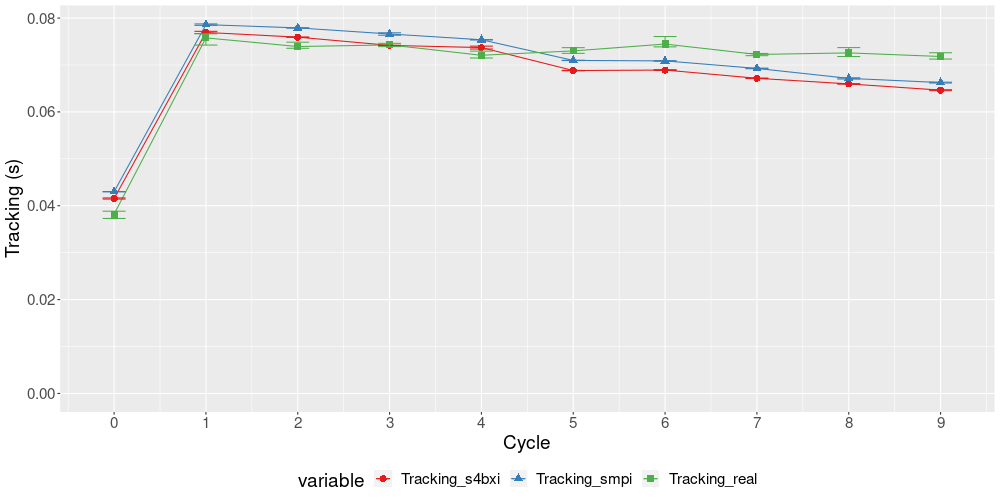
\includegraphics[width=1\textwidth]{5_high_level/Quicksilver/10000particles_4tasks_1ppn.png}
    \caption{Quiksilver experiment on 10,000 particles, with 4 nodes and 1 process per node}
    \label{fig:5_high_level:quicksilver_4tasks_1ppn}
\end{figure}


With very small cluster sizes, we can see that both simulators continue to have
a good accuracy. For example,
Figure~\ref{fig:5_high_level:quicksilver_4tasks_1ppn} shows the result of
executing Quicksilver on four nodes, with one process per node, and still 10,000
input particles.


\begin{figure}[!tb]
    \centering
    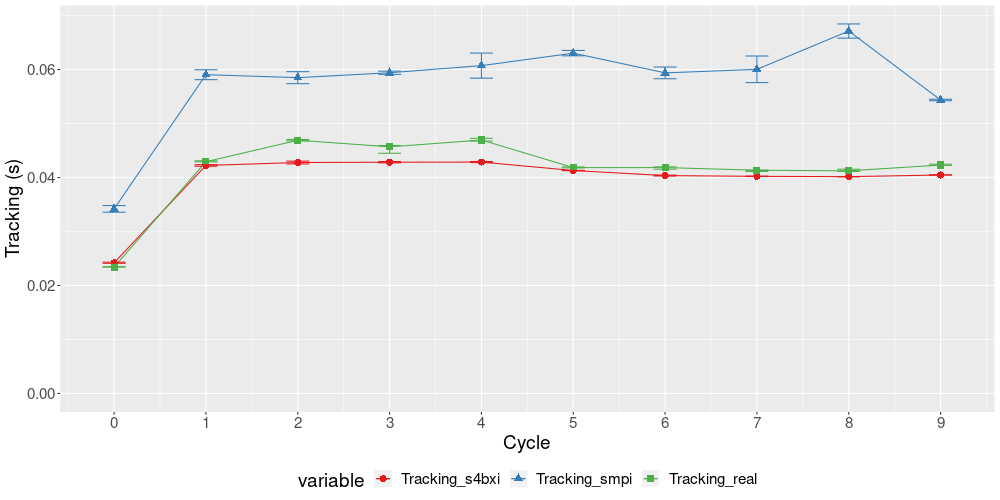
\includegraphics[width=1\textwidth]{5_high_level/Quicksilver/10000particles_8tasks_1ppn.png}
    \caption{Quiksilver experiment on 10,000 particles, with 8 nodes and 1 process per node}
    \label{fig:5_high_level:quicksilver_8tasks_1ppn}
\end{figure}

On the other hand, as soon as we use more than 8 MPI ranks (regardless of the
number of nodes), we observe a quick degradation of the accuracy of SMPI, while
OpenMPI over S4BXI keeps a good accuracy. We can see the start of this trend
with an execution on eight nodes and one process per node on
Figure~\ref{fig:5_high_level:quicksilver_8tasks_1ppn}. It only gets worse for
larger numbers of MPI ranks, as we can see on
Figure~\ref{fig:5_high_level:quicksilver_16tasks_1ppn} for 16 nodes and one
process per node, or Figure~\ref{fig:5_high_level:quicksilver_16tasks_4ppn} for
four nodes and four processes per node (so 16 processes in total again).


\begin{figure}[!tb]
    \centering
    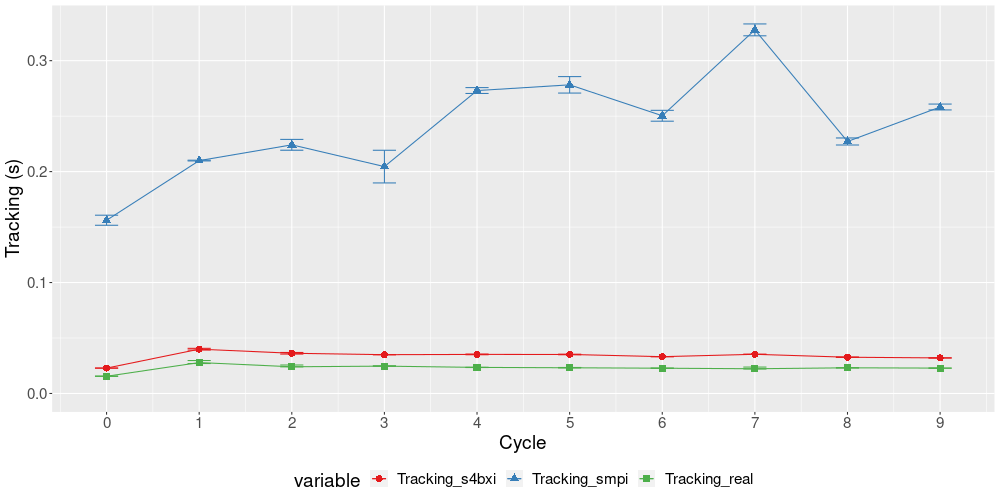
\includegraphics[width=1\textwidth]{5_high_level/Quicksilver/10000particles_16tasks_1ppn.png}
    \caption{Quiksilver experiment on 10,000 particles, with 16 nodes and 1 process per node}
    \label{fig:5_high_level:quicksilver_16tasks_1ppn}
\end{figure}

\begin{figure}[!tb]
    \centering
    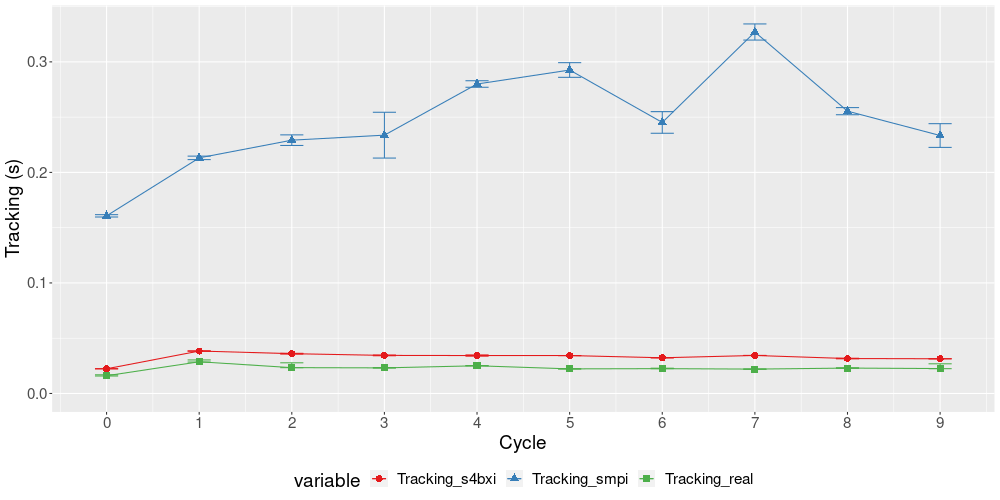
\includegraphics[width=1\textwidth]{5_high_level/Quicksilver/10000particles_16tasks_4ppn.png}
    \caption{Quiksilver experiment on 10,000 particles, with 4 nodes and 4 processes per node}
    \label{fig:5_high_level:quicksilver_16tasks_4ppn}
\end{figure}

As we increase the number of particles given as an input to Quicksilver, we can
observe the same phenomenon. The only difference is that as we increase the
problem size, SMPI remains accurate for larger cluster sizes, but we always
observe a point where SMPI's accuracy drops dramatically. For example, with
1,000,000 particles, we conserve a good accuracy of both simulators up to 16 MPI
ranks, as we can see on Figure~\ref{fig:5_high_level:quicksilver_16tasks_2ppn}
(with eight nodes and two process per node). Starting from 32 MPI ranks, we can
see the accuracy of SMPI drops, for example on
Figure~\ref{fig:5_high_level:quicksilver_32tasks_2ppn}.

\begin{figure}[!tb]
    \centering
    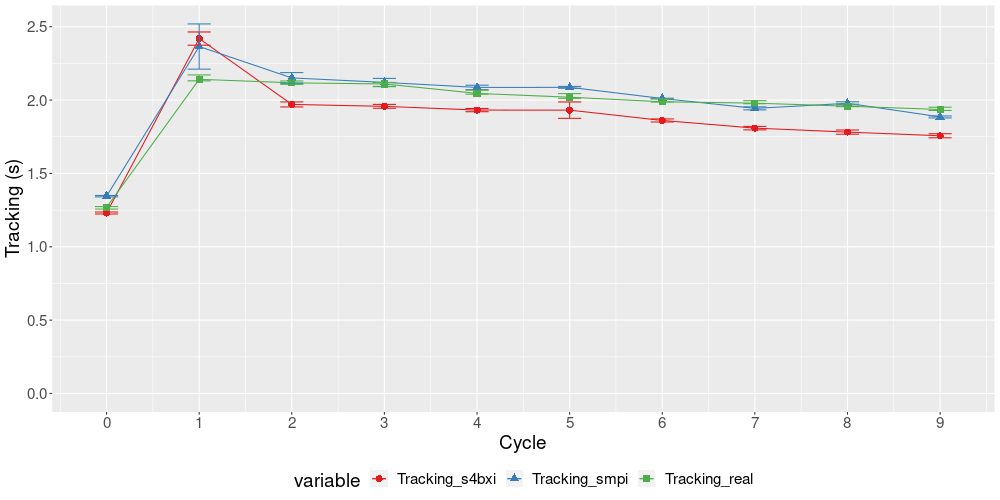
\includegraphics[width=1\textwidth]{5_high_level/Quicksilver/1000000particles_16tasks_2ppn.png}
    \caption{Quiksilver experiment on 1,000,000 particles, with 8 nodes and 2 processes per node}
    \label{fig:5_high_level:quicksilver_16tasks_2ppn}
\end{figure}

\begin{figure}[!tb]
    \centering
    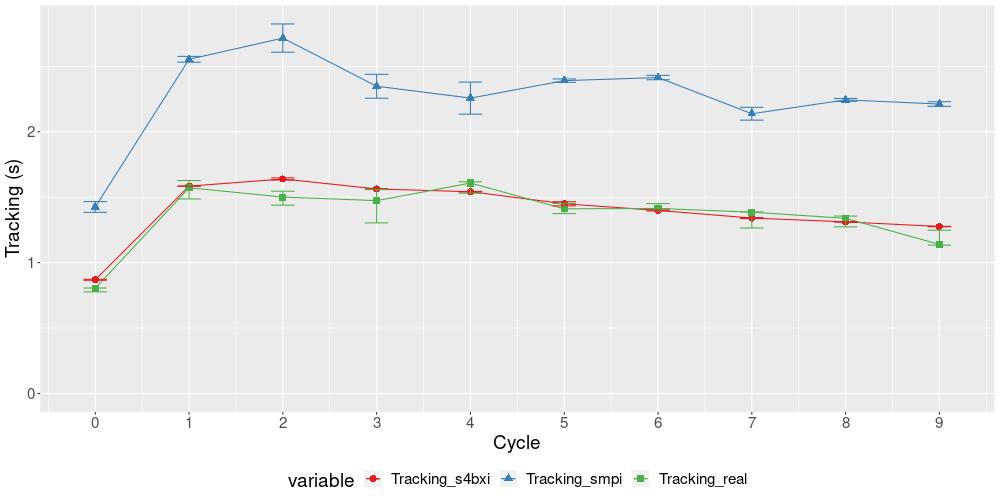
\includegraphics[width=1\textwidth]{5_high_level/Quicksilver/1000000particles_32tasks_2ppn.png}
    \caption{Quiksilver experiment on 1,000,000 particles, with 16 nodes and 2 processes per node}
    \label{fig:5_high_level:quicksilver_32tasks_2ppn}
\end{figure}

This lack of accuracy from SMPI is highly unexpected, as we never obtained
results so far away from the real-world experiment in OSU benchmarks or LULESH.
We were not able to identify what could be so detrimental to the SMPI model in
Quicksilver, only that the accuracy drop is very consistent, and depends on the
problem size and the number of MPI ranks, regardless of the number of nodes they
are distributed on.

\subsection{High-Performance Linpack (HPL)}

Finally, we tested our simulator on HPL. This application is particularly
interesting to study because we can use two different versions: in addition to
the ``regular'' version of HPL, we can use a skeleton version of the
application, made by Tom \textsc{Cornebize} during his PhD~\cite{Cornebize2021}.
The idea behind this version of HPL is that it performs the same communications
as the full application, but it replaces the most costly computation phases with
a delay that estimates the corresponding CPU time and which is simulated
instantaneously. The skeleton version does not compute the same result as the
original application but its simulated execution time is approximately the same.
In practice, the vast majority of the CPU time of the benchmark is spent in one
function (\inline{HPL_dgemm}), which performs a Double precision GEneral Matrix
Multiply (DGEMM). Therefore, we can save a lot of time in simulation be removing
the code of this function, and by replacing it with a function call to our
simulator in order to inject an artificial amount of computation time in the
model directly. Of course, this skeleton version of HPL does not perform
accurate computations, as many CPU operations were removed, but the timing of
HPL in simulated time is preserved because the operations that we removed do not
affect the execution flow of HPL.

\begin{figure}[!ht]
    \centering
    \includegraphicsOverflow{5_high_level/HPL/vanilla/__2nodes_1ppn_chap_5.png}{1.1}
    \caption{HPL experiment on 2 nodes with 1 process per node}
    \label{fig:5_high_level:hpl_vanilla_2x1}
\end{figure}

We will start by presenting our results for the full version of the application:
Figure~\ref{fig:5_high_level:hpl_vanilla_2x1} shows data from both simulators
(SMPI and OpenMPI over S4BXI) compared to real-world executions, for a very
small number of MPI ranks: two nodes with only one process per node. The left
graph shows the precision of the simulators, by plotting the performance
reported by HPL (in GFlops), whereas the right graph plots the performance of
the simulators (with respect to wall-clock time), compared to the duration of
the real-world experiment. We can see that even though the real-world
experiments show a surprising evolution of the computing power (in Gflops) when
the problem size increases, both simulators manage to model these effects
accurately. As the number of processes is very small, we can see that the
performance of both simulators is reasonably good, and that for large problem
sizes they perform very similarly.

\begin{figure}[!ht]
    \centering
    \includegraphicsOverflow{5_high_level/HPL/vanilla/__10nodes_5ppn_chap_5.png}{1.1}
    \caption{HPL experiment on 50 MPI ranks (10 nodes with 5 processes per node)}
    \label{fig:5_high_level:hpl_vanilla_10x5}
\end{figure}

\begin{figure}[!ht]
    \centering
    \includegraphicsOverflow{5_high_level/HPL/vanilla/__16nodes_8ppn_chap_5.png}{1.1}
    \caption{HPL experiment on 128 MPI ranks (16 nodes with 8 processes per node)}
    \label{fig:5_high_level:hpl_vanilla_16x8}
\end{figure}


\begin{figure}[!th]
    \centering
    \includegraphicsOverflow{5_high_level/HPL/optimized_grid5000_tuning/__2nodes_1ppn_chap_5.png}{1.1}
    \caption{HPL skeleton experiment on 2 nodes with 1 process per node}
    \label{fig:5_high_level:hpl_optimized_2x1_grid5000}
\end{figure}

\begin{figure}[!th]
    \centering
    \includegraphicsOverflow{5_high_level/HPL/optimized_grid5000_tuning/__10nodes_5ppn_chap_5.png}{1.1}
    \caption{HPL skeleton experiment on 50 MPI ranks (10 nodes with 5 processes per node)}
    \label{fig:5_high_level:hpl_optimized_10x5_grid5000}
\end{figure}

Executions with more MPI ranks are displayed on
Figure~\ref{fig:5_high_level:hpl_vanilla_10x5} for 50 MPI ranks (ten nodes and
five processes per node) and on Figure~\ref{fig:5_high_level:hpl_vanilla_16x8}
for 128 MPI ranks (16 nodes and eight processes per node). On both figures we
can see that the accuracy of the simulators is comparable, with a slight
advantage for SMPI. This result is not surprising, because of how HPL uses MPI:
even though the benchmark needs to be able to perform collective communications,
it does not use the collective primitives offered by MPI. Instead, all
operations are re-implemented in HPL with a combination of basic ``send'' and
``receive'' point-to-point primitives. Since SMPI's network model is
specifically tuned to perform well on these point-to-point operations (using
coefficients on the latency and bandwidth of Links), it is expected to get good
results in this context. In comparison, OpenMPI over S4BXI models low-level
network operations, which also gives good results. Nevertheless, in order to
surpass the accuracy of SMPI on this type of workload, our approach would
require a finer tuning of very low-level parameters inside our simulator. From a
performance perspective, as expected the duration of simulation increases with
the number of simulated MPI ranks. We can see that the gap between the
performance of SMPI and OpenMPI over S4BXI increases when we simulate more MPI
ranks, as we can see in Figure~\ref{fig:5_high_level:hpl_vanilla_2x1} where both
simulators are extremely close, whereas the gap is a lot more important on
figures~\ref{fig:5_high_level:hpl_vanilla_10x5}
and~\ref{fig:5_high_level:hpl_vanilla_16x8}. This different in scaling is
expected, since the proportion of network operations (compared to the
computational phases) increases as well, and modelling communications is more
costly with our approach than SMPI (which has a more simplistic network model).

\begin{figure}[!th]
    \centering
    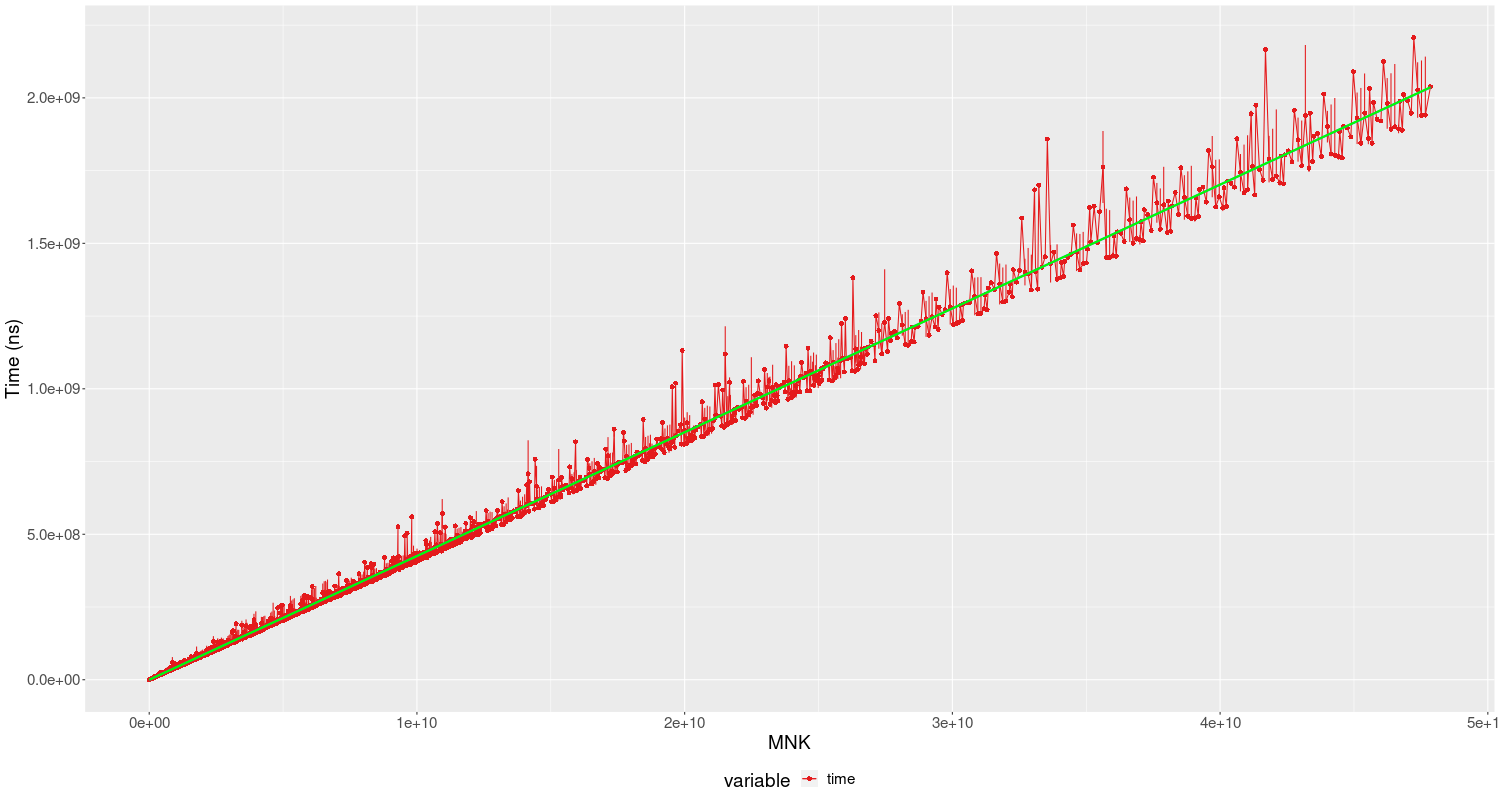
\includegraphics[width = 1\textwidth]{5_high_level/HPL/tuning/MNK.png}
    \caption{Duration of \inline{HPL_dgemm} as a function of $M \times N \times K$}
    \label{fig:5_high_level:hpl_optimized_MNK}
\end{figure}

\begin{figure}[!th]
    \centering
    \includegraphicsOverflow{5_high_level/HPL/4x4_no_vader_144_optimized_tuned.png}{1.1}
    \caption{HPL skeleton experiment on 16 MPI ranks (4 nodes with 4 processes per node), with our tuning}
    \label{fig:5_high_level:hpl_optimized_4x4}
\end{figure}

In order to improve the performance of the simulators, we can use the skeleton
version at our disposal. However, the main difficulty is to tune the artificial
computation time to inject in SimGrid (in the \inline{HPL_dgemm} function). In
his PhD, Tom \textsc{Cornebize} uses machines from the Grid5000 testbed, and we
re-used his tuning without any modifications at first. Results are depicted on
Figure~\ref{fig:5_high_level:hpl_optimized_2x1_grid5000} for two MPI ranks (two
nodes and one process per node) and on
Figure~\ref{fig:5_high_level:hpl_optimized_10x5_grid5000} for 50 MPI ranks (ten
nodes and five processes per node). From a performance perspective, we can see
that both simulators are sped up significantly (the SMPI simulation on two MPI
ranks is even faster than the real world experiment for all problem sizes). Of
course, the gap between the execution time of the simulators stays significant,
as the network model of our approach is still costly on the skeleton version (as
the number of communications is identical). Regarding accuracy, we can see that
this version of HPL (with this tuning) made both simulators very pessimistic,
which shows that the CPUs on our clusters are much more efficient at running
DGEMM operations than Grid5000's ones.


\begin{figure}[!ht]
    \centering
    \includegraphicsOverflow{5_high_level/HPL/4x4_no_vader_144_vanilla.png}{1.1}
    \caption{Full HPL experiment on 16 MPI ranks (4 nodes with 4 processes per node)}
    \label{fig:5_high_level:hpl_vanilla_4x4}
\end{figure}

To get a better tuning of our DGEMM model, we instrumented the real-world
version of HPL to measure the duration of the \inline{HPL_dgemm} primitive as a
function of its numerical parameters (which are called $M$, $N$ and $K$). By
plotting the performance of \inline{HPL_dgemm} as a function of each combination
of the parameters ($M$, $N$, $K$, $M \times N$, $M \times K$, $N \times K$ and
$M \times N \times K$), we identified that the execution time of
\inline{HPL_dgemm} seems close to a linear function of $M \times N \times K$
(with a significant amount of noise):
Figure~\ref{fig:5_high_level:hpl_optimized_MNK} shows this data, depicted along
with the corresponding linear regression. Consequently, we managed to tune the
estimation of the computation time; this allowed us to get the results depicted
on Figure~\ref{fig:5_high_level:hpl_optimized_4x4}. The corresponding run of the
full benchmark (on 16 MPI ranks) is shown on
Figure~\ref{fig:5_high_level:hpl_vanilla_4x4}. As we can see, even if our
heuristic to estimate the duration of \inline{HPL_dgemm} is better adapted to
our cluster, it is still far from perfect. This is expected since our tuning is
more simplistic than the study conducted by Tom \textsc{Cornebize}.

The most important takeaway from these experiments is that this type of skeleton
application, originally designed for SMPI, is fully compatible with S4BXI
simulations out of the box. Even though the improvement in performance is not as
important with our model as it is with SMPI, we showed that this type of patch
to an application works in an identical way in S4BXI and SMPI, as we can see
from the accuracy graphs.

\section{OpenSHMEM}

While modeling MPI is the main usage of our simulator, one of the strengths of
S4BXI is its adaptability: since it is modeling a low-level API, it can be used
to run a variety of higher-level APIs. To demonstrate that, we have worked on
the simulation of the OpenSHMEM library.

\subsection{Running OpenSHMEM in S4BXI}

OpenSHMEM follows a Partitioned global address space (PGAS) model, which means
that, compared to MPI, it focuses less on message passing. Instead, it gives
every process in the job a transparent view of a ``global memory pool'', which
in practice is distributed across several nodes. For our study we adapted Atos's
version of OpenSHMEM to support running on S4BXI. The Atos version is very
similar to Sandia's implementation of OpenSHMEM
(\url{https://github.com/Sandia-OpenSHMEM/SOS}), with only minor modifications
to support execution over BXI.

Similarly to OpenMPI, we chose to add support for OpenSHMEM simulation over
S4BXI by adding a small patch to OpenSHMEM. The architecture of OpenSHMEM's code
proved to be easier to work with for our purpose, because the project's scale is
significantly smaller, therefore making a preliminary patch to run this library
in simulation was much easier than the same developments in OpenMPI. In the end,
our patch simply adds a new file to OpenSHMEM, and the only modifications we
made to existing code was in the build scripts to include our new file.
Internally, OpenSHMEM uses a concept of a ``runtime'' that should be
initialized. The project natively provides four runtimes: one over MPI, and
three over various versions of PMI (PMI, PMI2 and PMIx). Therefore,  to add
support for S4BXI we only need a new runtime, which implements basic utilities
(like a barrier, basic metadata exchange), and we are ready to perform
simulations. This runtime only consists of 11 functions, most of which are
trivially implemented using S4BXI: the vast majority are implemented in one line
of code, and the largest one only has five lines of code. The full runtime is
given in Appendix~\ref{app:oshmem_code}.

Because of time constraints, and because our main goal was simulating MPI
accurately, we did not study OpenSHMEM benchmarks with as much detail as MPI
ones. The validation we performed focused on two aspects: the unit test suite
provided with OpenSHMEM, and the OSU-microbenchmarks (which also have an
OpenSHMEM variant even though the MPI benchmarks are more notorious).

\subsection{Experimental validation}

\begin{figure}[!b]
    \centering
    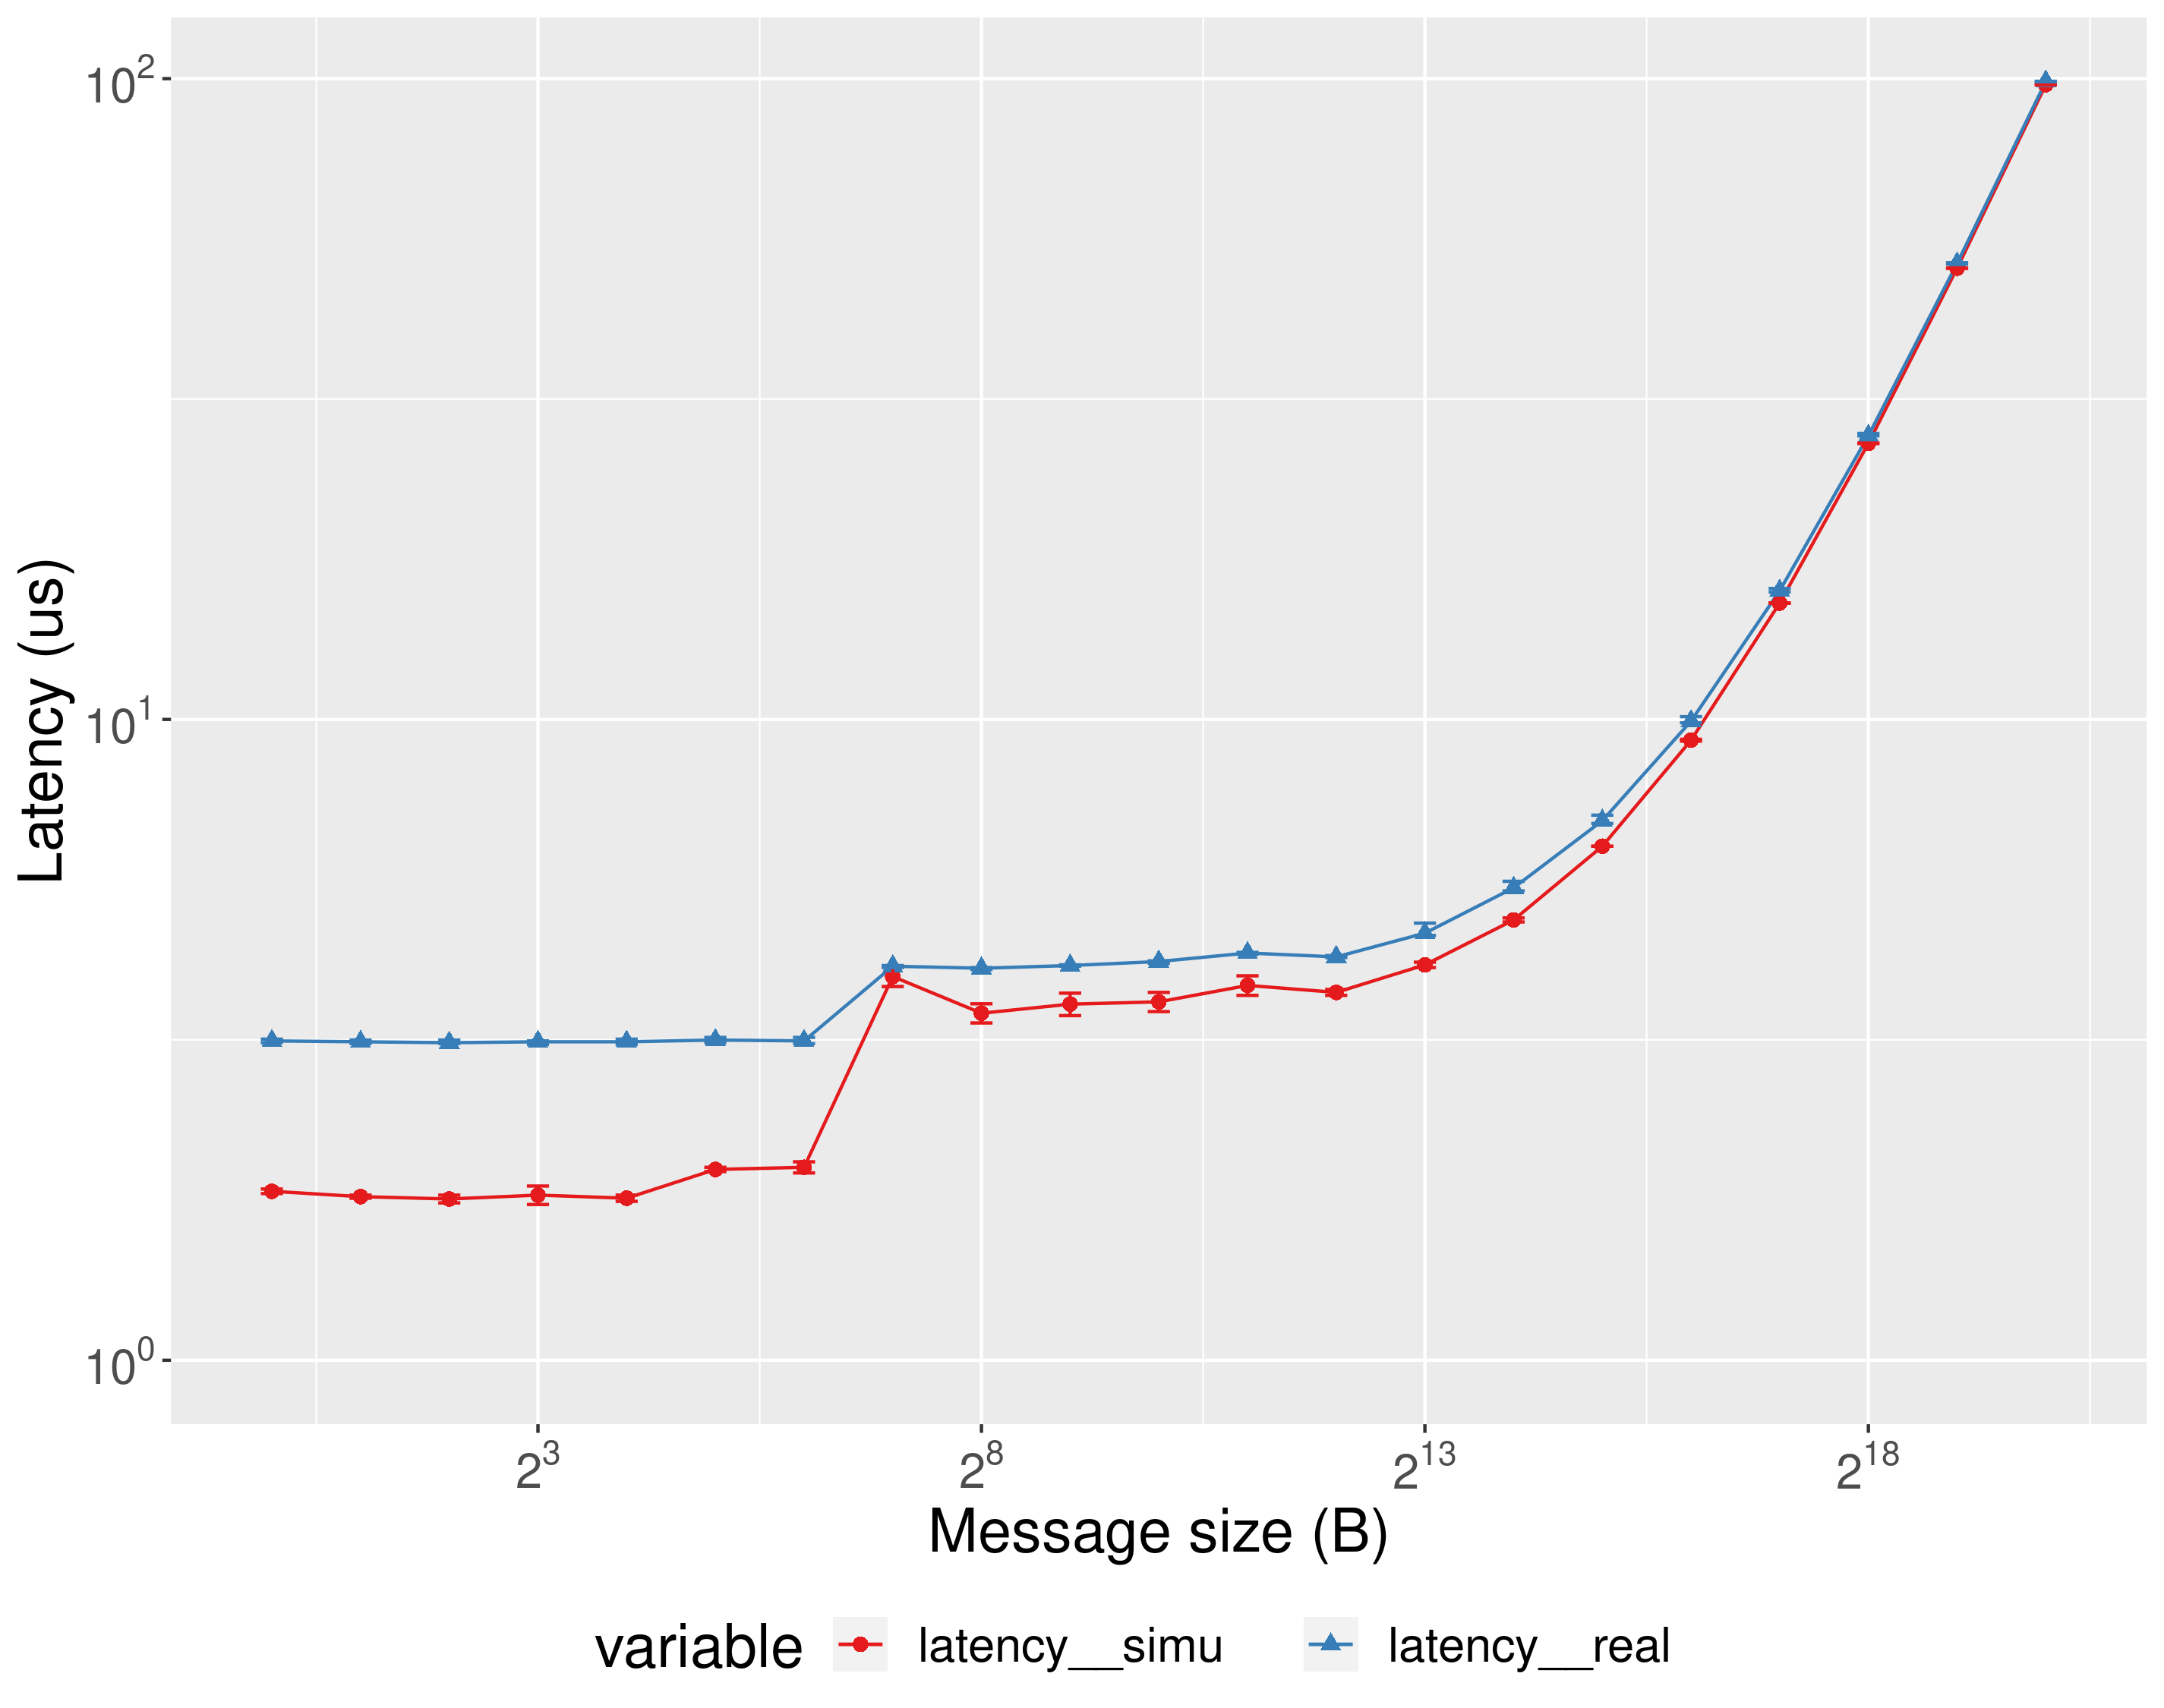
\includegraphics[width = 0.8\textwidth]{5_high_level/OpenSHMEM/put_2.png}
    \caption{Benchmark of the ``put'' operation of OpenSHMEM between 2 nodes}
    \label{fig:5_high_level:shmem_put}
\end{figure}

In order to test our simulations of OpenSHMEM, we first ran the unit test suite
provided by OpenSHMEM in our simulator, on a desktop computer. Every test was
executed four times: with 2, 4, 8 and 16 nodes and always one process per node,
this amounts to 392 runs in total. We used a fairly low value for the timeout,
of one minute, because we observed that most successful tests ran in a few
seconds only. The results are mixed: while the majority of tests pass -- 228
executions succeed -- we still have 154 errors, and 10 timeouts. Indeed, we
expected some tests to fail, as they perform operations that are not supported
by our simulators, such as using \inline{pthread} mutexes which are not properly
intercepted by S4BXI. However, the amount of errors is still a lot more
important than what we expected, and too large  to reliably run OpenSHMEM in
simulation. Nevertheless, these results show that with few efforts we are
already close to having a functional OpenSHMEM simulator, as most basic tests
work as expected.

\begin{figure}[!h]
    \centering
    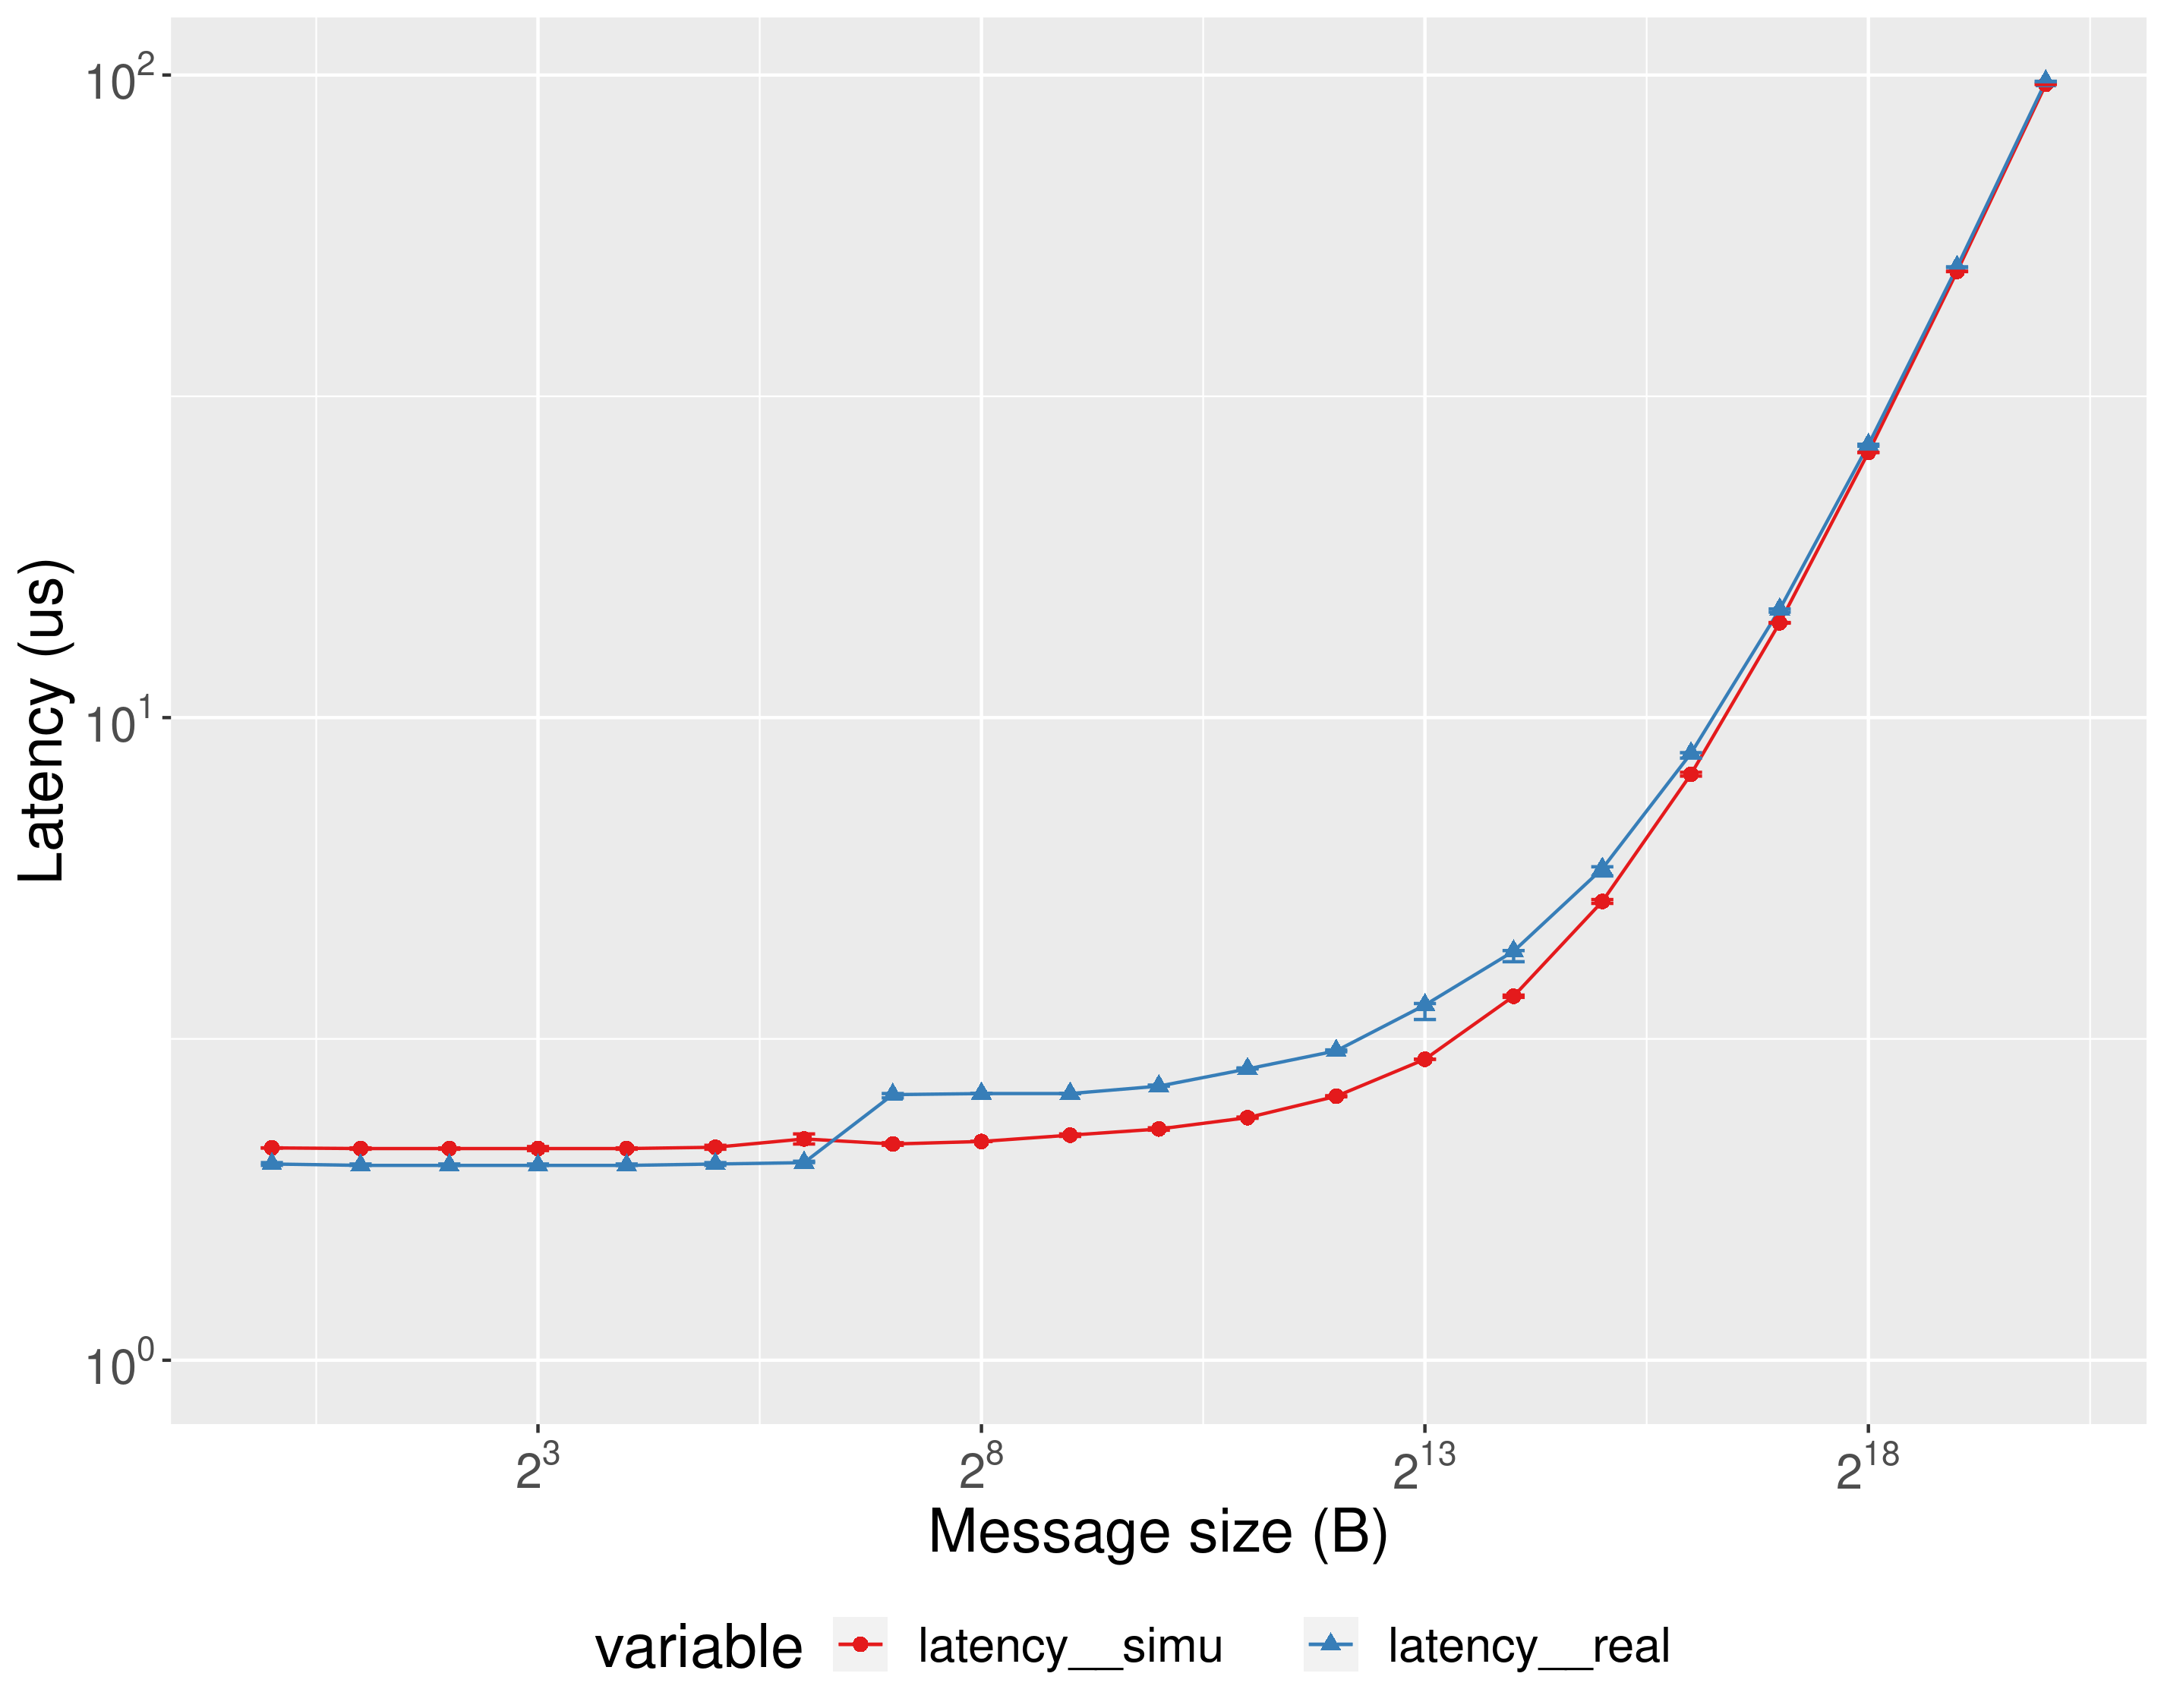
\includegraphics[width = 0.8\textwidth]{5_high_level/OpenSHMEM/get_2.png}
    \caption{Benchmark of the ``get'' operation of OpenSHMEM between 2 nodes}
    \label{fig:5_high_level:shmem_get}
\end{figure}

Running OpenSHMEM was only a side experiment in this thesis, and we did not
invest the time required to fully debug the problems. The only hypothesis that
we have is that OpenSHMEM tries to locate memory regions inside the current
binary at startup, which might cause problems in simulation since we do not
execute applications directly from their binary, but instead we run them from a
shared library which is opened by our entry point, \inline{s4bximain}. In the
real-world, each process would be isolated by the operating system and deployed
on several machines, but in simulation OpenSHMEM might locate the same memory
region for all processes (by looking directly in \inline{s4bximain}) with no
isolation. This could cause issues but would require further investigations.

After running unit tests, we tried the OpenSHMEM variant of OSU benchmarks. Once
again, some tests do not terminate properly, therefore we only present a few of
those which work correctly, in order to give an idea of the precision that we
can expect out of OpenSHMEM simulation. For point to point operations, we can
see on Figure~\ref{fig:5_high_level:shmem_put} the result of the ``put''
benchmark between two nodes (which correspond to a remote write), and on
Figure~\ref{fig:5_high_level:shmem_get} we have a similar benchmark for the
``get'' operation (remote read). We can see that the accuracy is not perfect,
especially for ``put'' operations of a small size, but overall it is already
acceptable, even though we did not perform any particular tuning to make
OpenSHMEM simulations more accurate.

\begin{figure}[!hb]
    \centering
    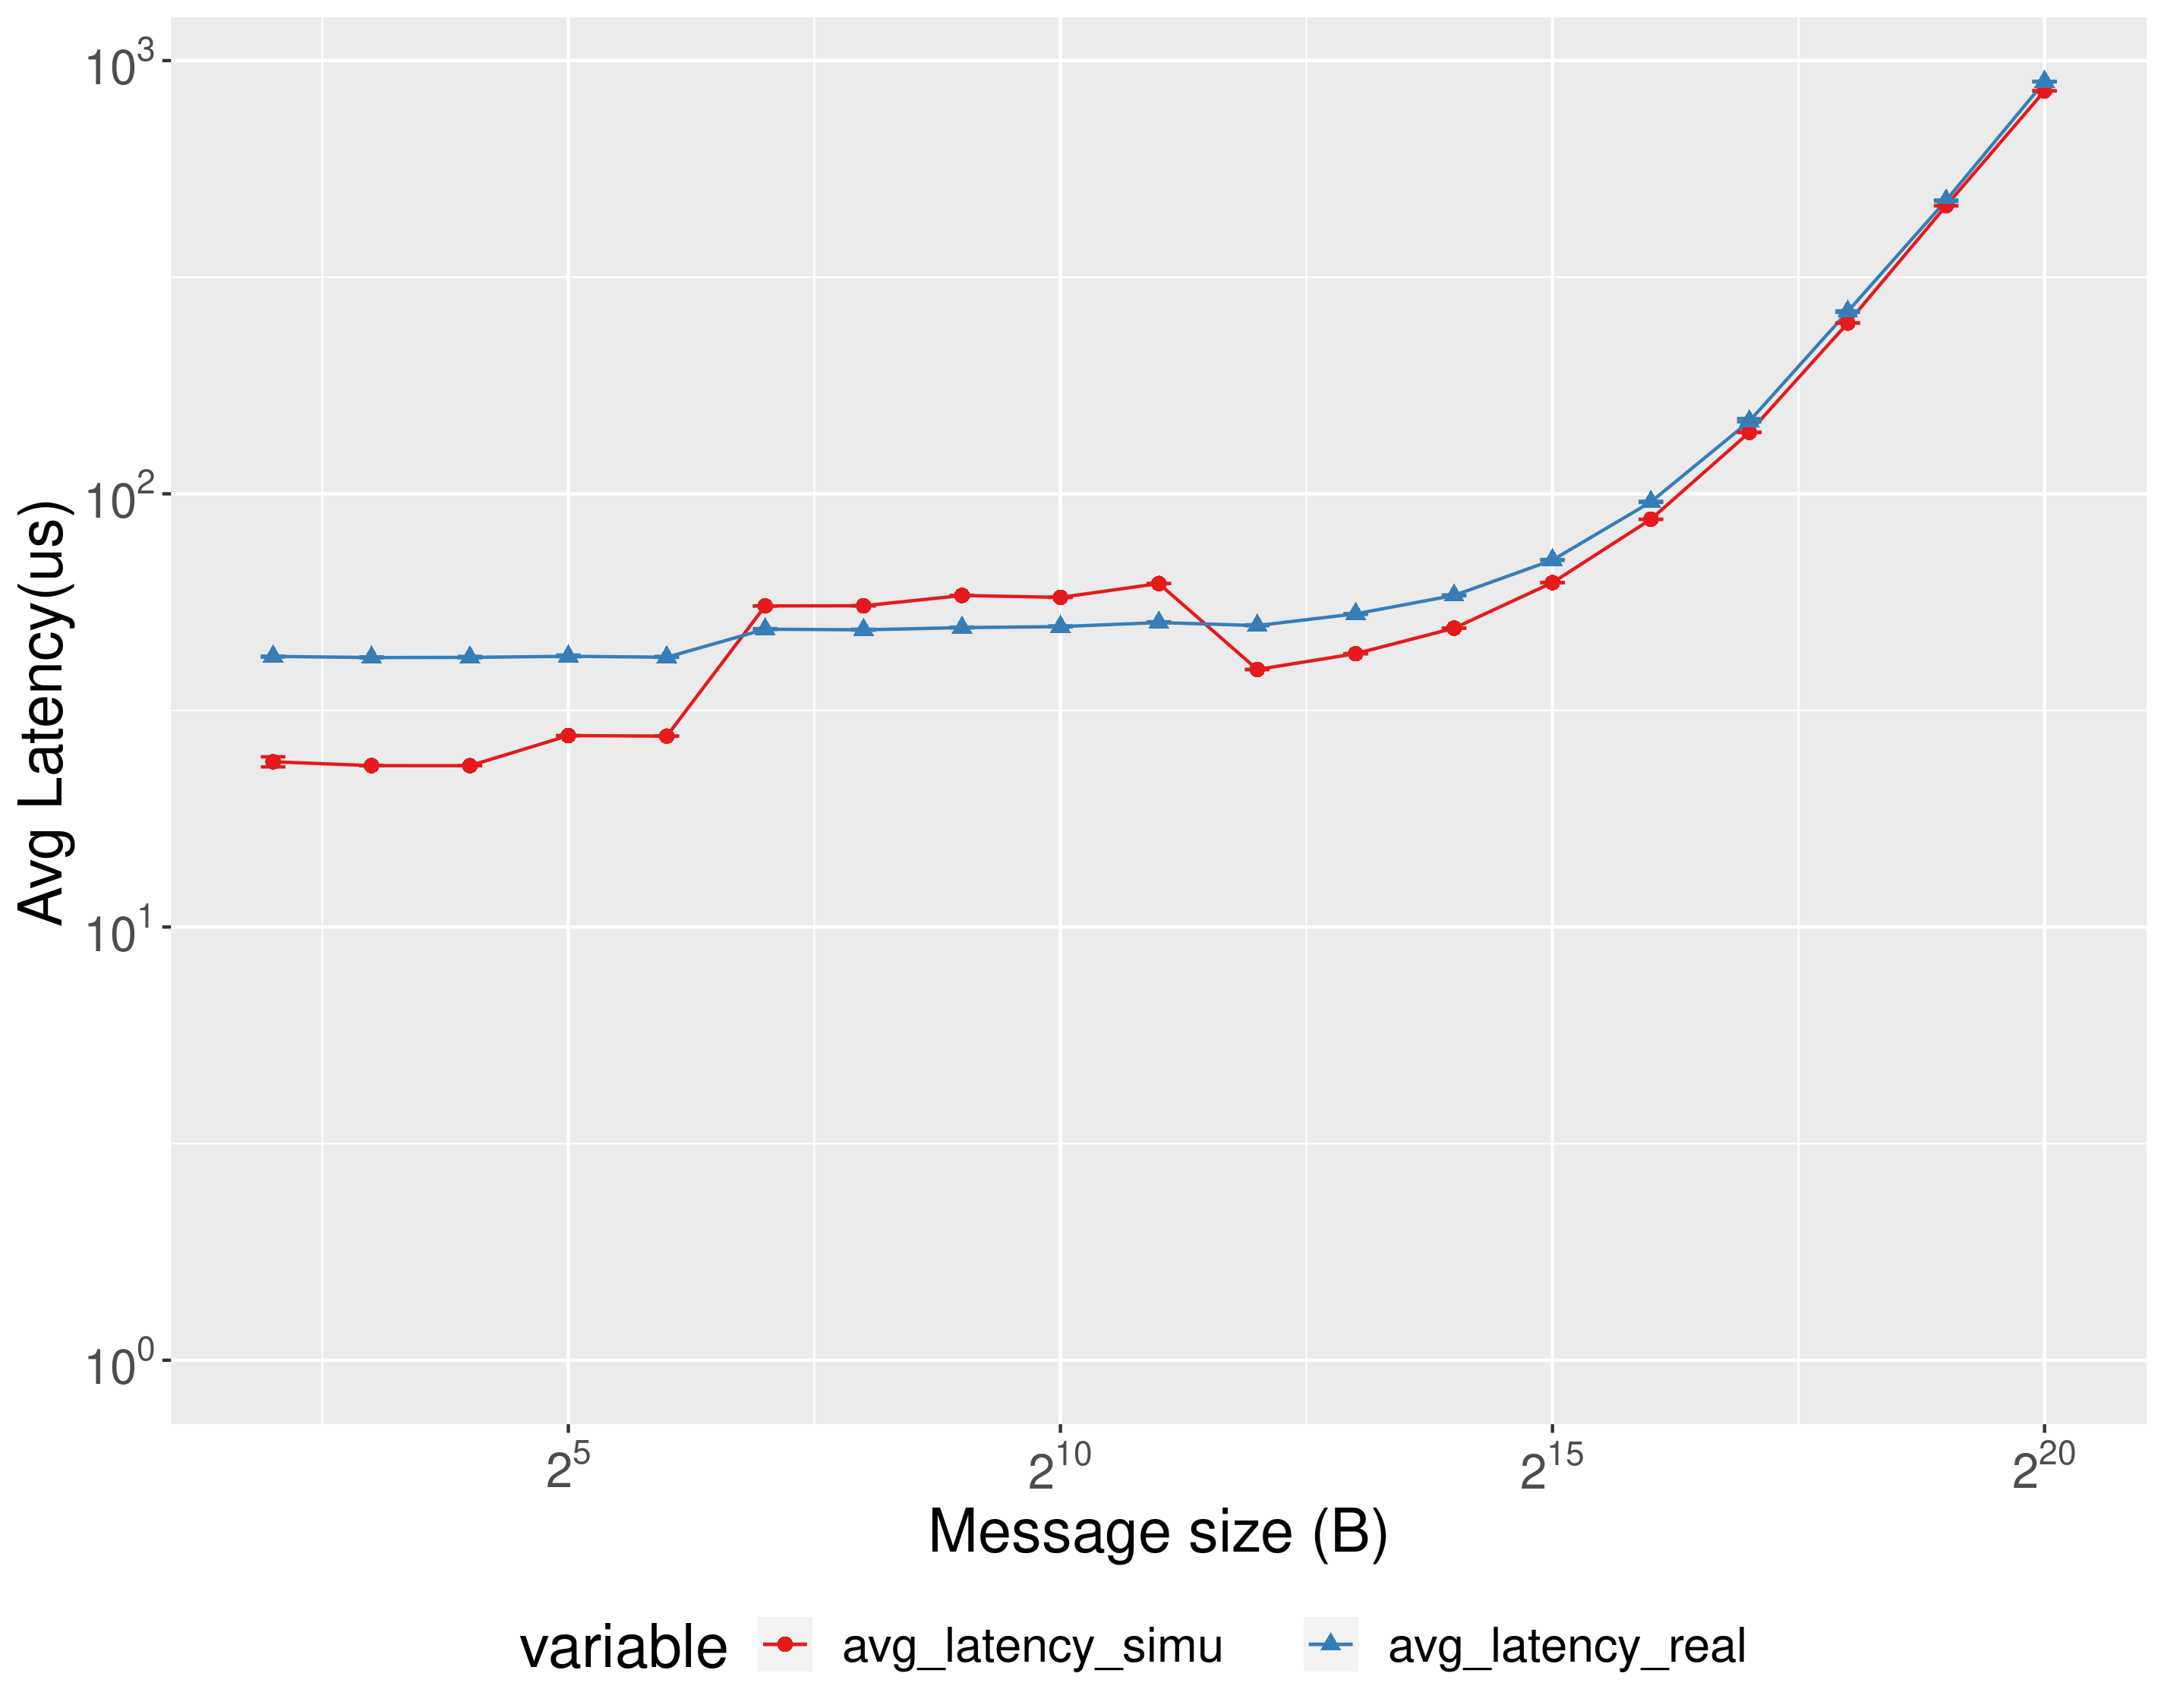
\includegraphics[width = 0.8\textwidth]{5_high_level/OpenSHMEM/fcollect_8.png}
    \caption{Benchmark of the ``fcollect'' operation of OpenSHMEM using 8 nodes}
    \label{fig:5_high_level:shmem_fcollect}
\end{figure}

\begin{figure}[!hb]
    \centering
    \includegraphics[width = 0.8\textwidth]{5_high_level/OpenSHMEM/reduce_16.png}
    \caption{``Reduce'' OSU benchmark using 16 nodes}
    \label{fig:5_high_level:shmem_reduce}
\end{figure}

For collective operations, we can see on
Figure~\ref{fig:5_high_level:shmem_fcollect} the result of the ``fcollect''
benchmark on eight nodes, which concatenates data from multiple processes into a
buffer on every process of the job. Finally,
Figure~\ref{fig:5_high_level:shmem_reduce} shows the result of the ``reduce''
benchmark on 16 nodes, which performs various reduction operations (min, max and
sum) using data from all processes (similarly to MPI's reduce operation). We can
see that the conclusion is the same on collective operation than with
point-to-point ones: overall the accuracy is acceptable, even though in this
case we can see some unexpected performance jumps, that we did not investigate
because of a lack of time.

\section{Summary}

Simulating high-level APIs with our method has proved perfectly achievable, even
if some development time has been required. Even though our simulations are
slower than real-world experiments, they have other advantages: they only use
one CPU core, therefore exploring a vast parameter space can be done in parallel
with many simulations on one or several machines. Additionally, our simulations
can be used to test many scenarios, as high-level APIs are modeled with a high
fidelity (since we run them with few modifications).

Even though our results concern mainly MPI, our preliminary results with
OpenSHMEM show that our method can be adapted to other high-level API, making
S4BXI more versatile than most state-of-the-art simulators.
